\documentclass[twoside]{book}

% Packages required by doxygen
\usepackage{fixltx2e}
\usepackage{calc}
\usepackage{doxygen}
\usepackage[export]{adjustbox} % also loads graphicx
\usepackage{graphicx}
\usepackage[utf8]{inputenc}
\usepackage{makeidx}
\usepackage{multicol}
\usepackage{multirow}
\PassOptionsToPackage{warn}{textcomp}
\usepackage{textcomp}
\usepackage[nointegrals]{wasysym}
\usepackage[table]{xcolor}

% Font selection
\usepackage[T1]{fontenc}
\usepackage[scaled=.90]{helvet}
\usepackage{courier}
\usepackage{amssymb}
\usepackage{sectsty}
\renewcommand{\familydefault}{\sfdefault}
\allsectionsfont{%
  \fontseries{bc}\selectfont%
  \color{darkgray}%
}
\renewcommand{\DoxyLabelFont}{%
  \fontseries{bc}\selectfont%
  \color{darkgray}%
}
\newcommand{\+}{\discretionary{\mbox{\scriptsize$\hookleftarrow$}}{}{}}

% Page & text layout
\usepackage{geometry}
\geometry{%
  a4paper,%
  top=2.5cm,%
  bottom=2.5cm,%
  left=2.5cm,%
  right=2.5cm%
}
\tolerance=750
\hfuzz=15pt
\hbadness=750
\setlength{\emergencystretch}{15pt}
\setlength{\parindent}{0cm}
\setlength{\parskip}{3ex plus 2ex minus 2ex}
\makeatletter
\renewcommand{\paragraph}{%
  \@startsection{paragraph}{4}{0ex}{-1.0ex}{1.0ex}{%
    \normalfont\normalsize\bfseries\SS@parafont%
  }%
}
\renewcommand{\subparagraph}{%
  \@startsection{subparagraph}{5}{0ex}{-1.0ex}{1.0ex}{%
    \normalfont\normalsize\bfseries\SS@subparafont%
  }%
}
\makeatother

% Headers & footers
\usepackage{fancyhdr}
\pagestyle{fancyplain}
\fancyhead[LE]{\fancyplain{}{\bfseries\thepage}}
\fancyhead[CE]{\fancyplain{}{}}
\fancyhead[RE]{\fancyplain{}{\bfseries\leftmark}}
\fancyhead[LO]{\fancyplain{}{\bfseries\rightmark}}
\fancyhead[CO]{\fancyplain{}{}}
\fancyhead[RO]{\fancyplain{}{\bfseries\thepage}}
\fancyfoot[LE]{\fancyplain{}{}}
\fancyfoot[CE]{\fancyplain{}{}}
\fancyfoot[RE]{\fancyplain{}{\bfseries\scriptsize Generated by Doxygen }}
\fancyfoot[LO]{\fancyplain{}{\bfseries\scriptsize Generated by Doxygen }}
\fancyfoot[CO]{\fancyplain{}{}}
\fancyfoot[RO]{\fancyplain{}{}}
\renewcommand{\footrulewidth}{0.4pt}
\renewcommand{\chaptermark}[1]{%
  \markboth{#1}{}%
}
\renewcommand{\sectionmark}[1]{%
  \markright{\thesection\ #1}%
}

% Indices & bibliography
\usepackage{natbib}
\usepackage[titles]{tocloft}
\setcounter{tocdepth}{3}
\setcounter{secnumdepth}{5}
\makeindex

% Hyperlinks (required, but should be loaded last)
\usepackage{ifpdf}
\ifpdf
  \usepackage[pdftex,pagebackref=true]{hyperref}
\else
  \usepackage[ps2pdf,pagebackref=true]{hyperref}
\fi
\hypersetup{%
  colorlinks=true,%
  linkcolor=blue,%
  citecolor=blue,%
  unicode%
}

% Custom commands
\newcommand{\clearemptydoublepage}{%
  \newpage{\pagestyle{empty}\cleardoublepage}%
}

\usepackage{caption}
\captionsetup{labelsep=space,justification=centering,font={bf},singlelinecheck=off,skip=4pt,position=top}

%===== C O N T E N T S =====

\begin{document}

% Titlepage & ToC
\hypersetup{pageanchor=false,
             bookmarksnumbered=true,
             pdfencoding=unicode
            }
\pagenumbering{alph}
\begin{titlepage}
\vspace*{7cm}
\begin{center}%
{\Large C\+O\+P-\/290 }\\
\vspace*{1cm}
{\large Generated by Doxygen 1.8.14}\\
\end{center}
\end{titlepage}
\clearemptydoublepage
\pagenumbering{roman}
\tableofcontents
\clearemptydoublepage
\pagenumbering{arabic}
\hypersetup{pageanchor=true}

%--- Begin generated contents ---
\chapter{Namespace Index}
\section{Namespace List}
Here is a list of all documented namespaces with brief descriptions\+:\begin{DoxyCompactList}
\item\contentsline{section}{\mbox{\hyperlink{namespace_n_graph}{N\+Graph}} \\*A mathematical graph object\+: a simple, directed, connected graph, where nodes are of arbitrary type (colores, cities, names, etc.) ~\newline
 Operations for adding and removing edges and vertices, together with functions for finding neighbors, subgraphs, and other properties are included }{\pageref{namespace_n_graph}}{}
\end{DoxyCompactList}

\chapter{Hierarchical Index}
\section{Class Hierarchy}
This inheritance list is sorted roughly, but not completely, alphabetically\+:\begin{DoxyCompactList}
\item \contentsline{section}{Edge}{\pageref{struct_edge}}{}
\item \contentsline{section}{Gnuplot}{\pageref{class_gnuplot}}{}
\item \contentsline{section}{Graph\+\_\+\+Imp}{\pageref{class_graph___imp}}{}
\item runtime\+\_\+error\begin{DoxyCompactList}
\item \contentsline{section}{Gnuplot\+Exception}{\pageref{class_gnuplot_exception}}{}
\end{DoxyCompactList}
\item \contentsline{section}{Show}{\pageref{class_show}}{}
\item \contentsline{section}{N\+Graph\+:\+:t\+Graph$<$ T $>$}{\pageref{class_n_graph_1_1t_graph}}{}
\item \contentsline{section}{Three\+\_\+\+D\+\_\+to\+\_\+\+Two\+\_\+D}{\pageref{class_three___d__to___two___d}}{}
\item \contentsline{section}{Triplet}{\pageref{struct_triplet}}{}
\item \contentsline{section}{Two\+\_\+\+D\+\_\+to\+\_\+\+Three\+\_\+D}{\pageref{class_two___d__to___three___d}}{}
\end{DoxyCompactList}

\chapter{Class Index}
\section{Class List}
Here are the classes, structs, unions and interfaces with brief descriptions\+:\begin{DoxyCompactList}
\item\contentsline{section}{\mbox{\hyperlink{struct_edge}{Edge}} \\*Defines a class for storing edges of the graph }{\pageref{struct_edge}}{}
\item\contentsline{section}{\mbox{\hyperlink{class_gnuplot}{Gnuplot}} }{\pageref{class_gnuplot}}{}
\item\contentsline{section}{\mbox{\hyperlink{class_gnuplot_exception}{Gnuplot\+Exception}} \\*A C++ interface to gnuplot }{\pageref{class_gnuplot_exception}}{}
\item\contentsline{section}{\mbox{\hyperlink{class_graph___imp}{Graph\+\_\+\+Imp}} \\*Defines a class for storing edges of the graph }{\pageref{class_graph___imp}}{}
\item\contentsline{section}{\mbox{\hyperlink{class_show}{Show}} \\*This is the class which will be used to handle all function related to showing and rendering the graph }{\pageref{class_show}}{}
\item\contentsline{section}{\mbox{\hyperlink{class_n_graph_1_1t_graph}{N\+Graph\+::t\+Graph$<$ T $>$}} }{\pageref{class_n_graph_1_1t_graph}}{}
\item\contentsline{section}{\mbox{\hyperlink{class_three___d__to___two___d}{Three\+\_\+\+D\+\_\+to\+\_\+\+Two\+\_\+D}} \\*Class for doing all operations on 3D to 2D }{\pageref{class_three___d__to___two___d}}{}
\item\contentsline{section}{\mbox{\hyperlink{struct_triplet}{Triplet}} \\*Defines a class for storing triplets }{\pageref{struct_triplet}}{}
\item\contentsline{section}{\mbox{\hyperlink{class_two___d__to___three___d}{Two\+\_\+\+D\+\_\+to\+\_\+\+Three\+\_\+D}} \\*Defines a class needed to generate the 3D object from the 3 2D projections }{\pageref{class_two___d__to___three___d}}{}
\end{DoxyCompactList}

\chapter{Namespace Documentation}
\hypertarget{namespace_n_graph}{}\section{N\+Graph Namespace Reference}
\label{namespace_n_graph}\index{N\+Graph@{N\+Graph}}


A mathematical graph object\+: a simple, directed, connected graph, where nodes are of arbitrary type (colores, cities, names, etc.) ~\newline
 Operations for adding and removing edges and vertices, together with functions for finding neighbors, subgraphs, and other properties are included.  


\subsection*{Classes}
\begin{DoxyCompactItemize}
\item 
class \mbox{\hyperlink{class_n_graph_1_1t_graph}{t\+Graph}}
\end{DoxyCompactItemize}
\subsection*{Typedefs}
\begin{DoxyCompactItemize}
\item 
\mbox{\Hypertarget{namespace_n_graph_a397e01b6d7caaaf603e67c1a87f11048}\label{namespace_n_graph_a397e01b6d7caaaf603e67c1a87f11048}} 
typedef \mbox{\hyperlink{class_n_graph_1_1t_graph}{t\+Graph}}$<$ unsigned int $>$ {\bfseries Graph}
\item 
\mbox{\Hypertarget{namespace_n_graph_a00343a4aa68bb7a338a89a778942701f}\label{namespace_n_graph_a00343a4aa68bb7a338a89a778942701f}} 
typedef \mbox{\hyperlink{class_n_graph_1_1t_graph}{t\+Graph}}$<$ int $>$ {\bfseries i\+Graph}
\item 
\mbox{\Hypertarget{namespace_n_graph_a7b2d8922d00fae3af037b172b39fd524}\label{namespace_n_graph_a7b2d8922d00fae3af037b172b39fd524}} 
typedef \mbox{\hyperlink{class_n_graph_1_1t_graph}{t\+Graph}}$<$ std\+::string $>$ {\bfseries s\+Graph}
\end{DoxyCompactItemize}
\subsection*{Functions}
\begin{DoxyCompactItemize}
\item 
\mbox{\Hypertarget{namespace_n_graph_a619633fcec087680ab8d90510eade326}\label{namespace_n_graph_a619633fcec087680ab8d90510eade326}} 
{\footnotesize template$<$typename T $>$ }\\std\+::istream \& {\bfseries operator$>$$>$} (std\+::istream \&s, \mbox{\hyperlink{class_n_graph_1_1t_graph}{t\+Graph}}$<$ T $>$ \&G)
\item 
\mbox{\Hypertarget{namespace_n_graph_a8118891761ec5e37cfd25efa666c73d8}\label{namespace_n_graph_a8118891761ec5e37cfd25efa666c73d8}} 
{\footnotesize template$<$typename T $>$ }\\std\+::ostream \& {\bfseries operator$<$$<$} (std\+::ostream \&s, const \mbox{\hyperlink{class_n_graph_1_1t_graph}{t\+Graph}}$<$ T $>$ \&G)
\end{DoxyCompactItemize}


\subsection{Detailed Description}
A mathematical graph object\+: a simple, directed, connected graph, where nodes are of arbitrary type (colores, cities, names, etc.) ~\newline
 Operations for adding and removing edges and vertices, together with functions for finding neighbors, subgraphs, and other properties are included. 

Example\+:


\begin{DoxyPre}
    enum color \{blue, green, red, yellow, pink, black\};
    tGraph<color> A;\end{DoxyPre}



\begin{DoxyPre}    A.insert\_edge(blue, red);
    A.insert\_edge(yellow, blue);
    A.insert\_edge(blue, black);\end{DoxyPre}



\begin{DoxyPre}    tGraph<color> B(A), S=A.subgraph(blue);\end{DoxyPre}



\begin{DoxyPre}\end{DoxyPre}
 
\chapter{Class Documentation}
\hypertarget{struct_edge}{}\section{Edge Struct Reference}
\label{struct_edge}\index{Edge@{Edge}}


Data structure to store graph edges.  


\subsection*{Public Attributes}
\begin{DoxyCompactItemize}
\item 
\mbox{\Hypertarget{struct_edge_a9a415f211c059647d1b3af8fcf7a0e30}\label{struct_edge_a9a415f211c059647d1b3af8fcf7a0e30}} 
int {\bfseries src}
\item 
\mbox{\Hypertarget{struct_edge_ad7df434ff7710e69f28bb31e91a35f82}\label{struct_edge_ad7df434ff7710e69f28bb31e91a35f82}} 
int {\bfseries dest}
\end{DoxyCompactItemize}


\subsection{Detailed Description}
Data structure to store graph edges. 

The documentation for this struct was generated from the following file\+:\begin{DoxyCompactItemize}
\item 
/\+Users/sanjaybansal/\+Desktop/cop290/project/threeto2d.\+cpp\end{DoxyCompactItemize}

\hypertarget{class_gnuplot}{}\section{Gnuplot Class Reference}
\label{class_gnuplot}\index{Gnuplot@{Gnuplot}}
\subsection*{Public Member Functions}
\begin{DoxyCompactItemize}
\item 
\mbox{\Hypertarget{class_gnuplot_a187eb517b362cf379492fe7f1621ee50}\label{class_gnuplot_a187eb517b362cf379492fe7f1621ee50}} 
\mbox{\hyperlink{class_gnuplot_a187eb517b362cf379492fe7f1621ee50}{Gnuplot}} (const std\+::string \&style=\char`\"{}points\char`\"{})
\begin{DoxyCompactList}\small\item\em set a style during construction \end{DoxyCompactList}\item 
\mbox{\Hypertarget{class_gnuplot_a8ceac5808e42665c1dee305ae7ea9070}\label{class_gnuplot_a8ceac5808e42665c1dee305ae7ea9070}} 
\mbox{\hyperlink{class_gnuplot_a8ceac5808e42665c1dee305ae7ea9070}{Gnuplot}} (const std\+::vector$<$ double $>$ \&x, const std\+::string \&title=\char`\"{}\char`\"{}, const std\+::string \&style=\char`\"{}points\char`\"{}, const std\+::string \&labelx=\char`\"{}x\char`\"{}, const std\+::string \&labely=\char`\"{}y\char`\"{})
\begin{DoxyCompactList}\small\item\em plot a single std\+::vector at one go \end{DoxyCompactList}\item 
\mbox{\Hypertarget{class_gnuplot_a24327b6116c71acdc195eadf665c67cb}\label{class_gnuplot_a24327b6116c71acdc195eadf665c67cb}} 
\mbox{\hyperlink{class_gnuplot_a24327b6116c71acdc195eadf665c67cb}{Gnuplot}} (const std\+::vector$<$ double $>$ \&x, const std\+::vector$<$ double $>$ \&y, const std\+::string \&title=\char`\"{}\char`\"{}, const std\+::string \&style=\char`\"{}points\char`\"{}, const std\+::string \&labelx=\char`\"{}x\char`\"{}, const std\+::string \&labely=\char`\"{}y\char`\"{})
\begin{DoxyCompactList}\small\item\em plot pairs std\+::vector at one go \end{DoxyCompactList}\item 
\mbox{\Hypertarget{class_gnuplot_a14191e89154f2716608f6907975cc012}\label{class_gnuplot_a14191e89154f2716608f6907975cc012}} 
\mbox{\hyperlink{class_gnuplot_a14191e89154f2716608f6907975cc012}{Gnuplot}} (const std\+::vector$<$ double $>$ \&x, const std\+::vector$<$ double $>$ \&y, const std\+::vector$<$ double $>$ \&z, const std\+::string \&title=\char`\"{}\char`\"{}, const std\+::string \&style=\char`\"{}points\char`\"{}, const std\+::string \&labelx=\char`\"{}x\char`\"{}, const std\+::string \&labely=\char`\"{}y\char`\"{}, const std\+::string \&labelz=\char`\"{}z\char`\"{})
\begin{DoxyCompactList}\small\item\em plot triples std\+::vector at one go \end{DoxyCompactList}\item 
\mbox{\Hypertarget{class_gnuplot_a78a68f621caa87d1f34324fcd093c7bd}\label{class_gnuplot_a78a68f621caa87d1f34324fcd093c7bd}} 
\mbox{\hyperlink{class_gnuplot_a78a68f621caa87d1f34324fcd093c7bd}{$\sim$\+Gnuplot}} ()
\begin{DoxyCompactList}\small\item\em destructor\+: needed to delete temporary files \end{DoxyCompactList}\item 
\mbox{\Hypertarget{class_gnuplot_a07607803ede8dd5416906df0a1924fc5}\label{class_gnuplot_a07607803ede8dd5416906df0a1924fc5}} 
\mbox{\hyperlink{class_gnuplot}{Gnuplot}} \& \mbox{\hyperlink{class_gnuplot_a07607803ede8dd5416906df0a1924fc5}{cmd}} (const std\+::string \&cmdstr)
\begin{DoxyCompactList}\small\item\em send a command to gnuplot \end{DoxyCompactList}\item 
\mbox{\hyperlink{class_gnuplot}{Gnuplot}} \& \mbox{\hyperlink{class_gnuplot_afb69631c7a498077e378a3cbb56f38c8}{operator$<$$<$}} (const std\+::string \&cmdstr)
\begin{DoxyCompactList}\small\item\em Sends a command to an active gnuplot session, identical to \mbox{\hyperlink{class_gnuplot_a07607803ede8dd5416906df0a1924fc5}{cmd()}} send a command to gnuplot using the $<$$<$ operator. \end{DoxyCompactList}\item 
\mbox{\Hypertarget{class_gnuplot_a356d2faaa79f08d13fec9718b776b28d}\label{class_gnuplot_a356d2faaa79f08d13fec9718b776b28d}} 
\mbox{\hyperlink{class_gnuplot}{Gnuplot}} \& \mbox{\hyperlink{class_gnuplot_a356d2faaa79f08d13fec9718b776b28d}{showonscreen}} ()
\begin{DoxyCompactList}\small\item\em sets terminal type to terminal\+\_\+std \end{DoxyCompactList}\item 
\mbox{\Hypertarget{class_gnuplot_a032072c7c01b508a7535a17fb08562b1}\label{class_gnuplot_a032072c7c01b508a7535a17fb08562b1}} 
\mbox{\hyperlink{class_gnuplot}{Gnuplot}} \& \mbox{\hyperlink{class_gnuplot_a032072c7c01b508a7535a17fb08562b1}{savetops}} (const std\+::string \&filename=\char`\"{}gnuplot\+\_\+output\char`\"{})
\begin{DoxyCompactList}\small\item\em saves a gnuplot session to a postscript file, filename without extension \end{DoxyCompactList}\item 
\mbox{\hyperlink{class_gnuplot}{Gnuplot}} \& \mbox{\hyperlink{class_gnuplot_acfdcda292650775ebed4683e8e1515b5}{set\+\_\+style}} (const std\+::string \&stylestr=\char`\"{}points\char`\"{})
\item 
\mbox{\hyperlink{class_gnuplot}{Gnuplot}} \& \mbox{\hyperlink{class_gnuplot_aa18386919da2ec4c994f1f9c7195d384}{set\+\_\+smooth}} (const std\+::string \&stylestr=\char`\"{}csplines\char`\"{})
\item 
\mbox{\hyperlink{class_gnuplot}{Gnuplot}} \& \mbox{\hyperlink{class_gnuplot_ad9dfbccd66dece1dbe5803605c6ab08c}{unset\+\_\+smooth}} ()
\begin{DoxyCompactList}\small\item\em unset smooth attention\+: smooth is not set by default \end{DoxyCompactList}\item 
\mbox{\Hypertarget{class_gnuplot_a95ec1636a871447dfe99463b769339c7}\label{class_gnuplot_a95ec1636a871447dfe99463b769339c7}} 
\mbox{\hyperlink{class_gnuplot}{Gnuplot}} \& \mbox{\hyperlink{class_gnuplot_a95ec1636a871447dfe99463b769339c7}{set\+\_\+pointsize}} (const double pointsize=1.\+0)
\begin{DoxyCompactList}\small\item\em scales the size of the points used in plots \end{DoxyCompactList}\item 
\mbox{\Hypertarget{class_gnuplot_a5416c8e81f1b9945b9631fa85a8d4f47}\label{class_gnuplot_a5416c8e81f1b9945b9631fa85a8d4f47}} 
\mbox{\hyperlink{class_gnuplot}{Gnuplot}} \& \mbox{\hyperlink{class_gnuplot_a5416c8e81f1b9945b9631fa85a8d4f47}{set\+\_\+grid}} ()
\begin{DoxyCompactList}\small\item\em turns grid on/off \end{DoxyCompactList}\item 
\mbox{\Hypertarget{class_gnuplot_a53183e1487bc6977f0d46bf75d19b4d3}\label{class_gnuplot_a53183e1487bc6977f0d46bf75d19b4d3}} 
\mbox{\hyperlink{class_gnuplot}{Gnuplot}} \& \mbox{\hyperlink{class_gnuplot_a53183e1487bc6977f0d46bf75d19b4d3}{unset\+\_\+grid}} ()
\begin{DoxyCompactList}\small\item\em grid is not set by default \end{DoxyCompactList}\item 
\mbox{\hyperlink{class_gnuplot}{Gnuplot}} \& \mbox{\hyperlink{class_gnuplot_a67efc4d4dc46b6100d14ba2f7366ef11}{set\+\_\+multiplot}} ()
\item 
\mbox{\hyperlink{class_gnuplot}{Gnuplot}} \& \mbox{\hyperlink{class_gnuplot_aad76cdec16cfb5fdf82f45ed2786f4d8}{unset\+\_\+multiplot}} ()
\item 
\mbox{\Hypertarget{class_gnuplot_a671cbe7b18a267ea59f532c83a0035f6}\label{class_gnuplot_a671cbe7b18a267ea59f532c83a0035f6}} 
\mbox{\hyperlink{class_gnuplot}{Gnuplot}} \& \mbox{\hyperlink{class_gnuplot_a671cbe7b18a267ea59f532c83a0035f6}{set\+\_\+samples}} (const int samples=100)
\begin{DoxyCompactList}\small\item\em set sampling rate of functions, or for interpolating data \end{DoxyCompactList}\item 
\mbox{\Hypertarget{class_gnuplot_ab810fa4c02fb49ae197786c305b78702}\label{class_gnuplot_ab810fa4c02fb49ae197786c305b78702}} 
\mbox{\hyperlink{class_gnuplot}{Gnuplot}} \& \mbox{\hyperlink{class_gnuplot_ab810fa4c02fb49ae197786c305b78702}{set\+\_\+isosamples}} (const int isolines=10)
\begin{DoxyCompactList}\small\item\em set isoline density (grid) for plotting functions as surfaces (for 3d plots) \end{DoxyCompactList}\item 
\mbox{\hyperlink{class_gnuplot}{Gnuplot}} \& \mbox{\hyperlink{class_gnuplot_a891f9800705eddc3f73886f265c009b8}{set\+\_\+hidden3d}} ()
\item 
\mbox{\hyperlink{class_gnuplot}{Gnuplot}} \& \mbox{\hyperlink{class_gnuplot_ab8688182047f746090e1e5f2a8c11c9e}{unset\+\_\+hidden3d}} ()
\item 
\mbox{\hyperlink{class_gnuplot}{Gnuplot}} \& \mbox{\hyperlink{class_gnuplot_af845efc728a90d7e10de764eff0b2423}{set\+\_\+contour}} (const std\+::string \&position=\char`\"{}base\char`\"{})
\item 
\mbox{\hyperlink{class_gnuplot}{Gnuplot}} \& \mbox{\hyperlink{class_gnuplot_a0b8522cb81e46dd4f5a22b7b48f977b1}{unset\+\_\+contour}} ()
\item 
\mbox{\hyperlink{class_gnuplot}{Gnuplot}} \& \mbox{\hyperlink{class_gnuplot_a9825bd26500e30ca88404c4807e6607a}{set\+\_\+surface}} ()
\item 
\mbox{\hyperlink{class_gnuplot}{Gnuplot}} \& \mbox{\hyperlink{class_gnuplot_a4ebddacbec61aa3e7bc4b89f508ad621}{unset\+\_\+surface}} ()
\item 
\mbox{\hyperlink{class_gnuplot}{Gnuplot}} \& \mbox{\hyperlink{class_gnuplot_ad64a717dac18167f656c4f09239973f8}{set\+\_\+legend}} (const std\+::string \&position=\char`\"{}default\char`\"{})
\item 
\mbox{\hyperlink{class_gnuplot}{Gnuplot}} \& \mbox{\hyperlink{class_gnuplot_ace901a18ab1a459213afd3ee0233b5ce}{unset\+\_\+legend}} ()
\begin{DoxyCompactList}\small\item\em Switches legend off attention\+:legend is set by default. \end{DoxyCompactList}\item 
\mbox{\hyperlink{class_gnuplot}{Gnuplot}} \& \mbox{\hyperlink{class_gnuplot_a4f93bac0e69dd83806652ca7226c6b3b}{set\+\_\+title}} (const std\+::string \&title=\char`\"{}\char`\"{})
\begin{DoxyCompactList}\small\item\em sets and clears the title of a gnuplot session \end{DoxyCompactList}\item 
\mbox{\hyperlink{class_gnuplot}{Gnuplot}} \& \mbox{\hyperlink{class_gnuplot_aca0aeb1dc0ac8d7e68ba6a15a977be28}{unset\+\_\+title}} ()
\begin{DoxyCompactList}\small\item\em Clears the title of a gnuplot session The title is not set by default. \end{DoxyCompactList}\item 
\mbox{\Hypertarget{class_gnuplot_afcb311938827f8718f19ed52d66bad7c}\label{class_gnuplot_afcb311938827f8718f19ed52d66bad7c}} 
\mbox{\hyperlink{class_gnuplot}{Gnuplot}} \& \mbox{\hyperlink{class_gnuplot_afcb311938827f8718f19ed52d66bad7c}{set\+\_\+ylabel}} (const std\+::string \&label=\char`\"{}x\char`\"{})
\begin{DoxyCompactList}\small\item\em set x axis label \end{DoxyCompactList}\item 
\mbox{\Hypertarget{class_gnuplot_aa93589a95aeab869ba731e2583843ae4}\label{class_gnuplot_aa93589a95aeab869ba731e2583843ae4}} 
\mbox{\hyperlink{class_gnuplot}{Gnuplot}} \& \mbox{\hyperlink{class_gnuplot_aa93589a95aeab869ba731e2583843ae4}{set\+\_\+xlabel}} (const std\+::string \&label=\char`\"{}y\char`\"{})
\begin{DoxyCompactList}\small\item\em set y axis label \end{DoxyCompactList}\item 
\mbox{\Hypertarget{class_gnuplot_ab3206e715d20f05cc0dd1eec89ce8b07}\label{class_gnuplot_ab3206e715d20f05cc0dd1eec89ce8b07}} 
\mbox{\hyperlink{class_gnuplot}{Gnuplot}} \& \mbox{\hyperlink{class_gnuplot_ab3206e715d20f05cc0dd1eec89ce8b07}{set\+\_\+zlabel}} (const std\+::string \&label=\char`\"{}z\char`\"{})
\begin{DoxyCompactList}\small\item\em set z axis label \end{DoxyCompactList}\item 
\mbox{\Hypertarget{class_gnuplot_a4b8d96018f2d2d4e2922d4df153d6a84}\label{class_gnuplot_a4b8d96018f2d2d4e2922d4df153d6a84}} 
\mbox{\hyperlink{class_gnuplot}{Gnuplot}} \& \mbox{\hyperlink{class_gnuplot_a4b8d96018f2d2d4e2922d4df153d6a84}{set\+\_\+xrange}} (const double i\+From, const double i\+To)
\begin{DoxyCompactList}\small\item\em set axis -\/ ranges \end{DoxyCompactList}\item 
\mbox{\Hypertarget{class_gnuplot_a461271b7bfd4f84bdfc0055457226f28}\label{class_gnuplot_a461271b7bfd4f84bdfc0055457226f28}} 
\mbox{\hyperlink{class_gnuplot}{Gnuplot}} \& \mbox{\hyperlink{class_gnuplot_a461271b7bfd4f84bdfc0055457226f28}{set\+\_\+yrange}} (const double i\+From, const double i\+To)
\begin{DoxyCompactList}\small\item\em set y-\/axis -\/ ranges \end{DoxyCompactList}\item 
\mbox{\Hypertarget{class_gnuplot_a7273f6a48024117b4d234d0251106e78}\label{class_gnuplot_a7273f6a48024117b4d234d0251106e78}} 
\mbox{\hyperlink{class_gnuplot}{Gnuplot}} \& \mbox{\hyperlink{class_gnuplot_a7273f6a48024117b4d234d0251106e78}{set\+\_\+zrange}} (const double i\+From, const double i\+To)
\begin{DoxyCompactList}\small\item\em set z-\/axis -\/ ranges \end{DoxyCompactList}\item 
\mbox{\hyperlink{class_gnuplot}{Gnuplot}} \& \mbox{\hyperlink{class_gnuplot_a11a62a04c203f01607c3c21a727e318d}{set\+\_\+xautoscale}} ()
\item 
\mbox{\hyperlink{class_gnuplot}{Gnuplot}} \& \mbox{\hyperlink{class_gnuplot_a5b9e1a4e68f94d418a8e9194f168b448}{set\+\_\+yautoscale}} ()
\item 
\mbox{\hyperlink{class_gnuplot}{Gnuplot}} \& \mbox{\hyperlink{class_gnuplot_aef3e84e793836158e1ddd773d1465c37}{set\+\_\+zautoscale}} ()
\item 
\mbox{\Hypertarget{class_gnuplot_aff546fad227d93babeb5d2cc9f047b89}\label{class_gnuplot_aff546fad227d93babeb5d2cc9f047b89}} 
\mbox{\hyperlink{class_gnuplot}{Gnuplot}} \& \mbox{\hyperlink{class_gnuplot_aff546fad227d93babeb5d2cc9f047b89}{set\+\_\+xlogscale}} (const double base=10)
\begin{DoxyCompactList}\small\item\em turns on/off log scaling for the specified xaxis (logscale is not set by default) \end{DoxyCompactList}\item 
\mbox{\Hypertarget{class_gnuplot_a201a802d2f27fece0d39809c4eb3bce0}\label{class_gnuplot_a201a802d2f27fece0d39809c4eb3bce0}} 
\mbox{\hyperlink{class_gnuplot}{Gnuplot}} \& \mbox{\hyperlink{class_gnuplot_a201a802d2f27fece0d39809c4eb3bce0}{set\+\_\+ylogscale}} (const double base=10)
\begin{DoxyCompactList}\small\item\em turns on/off log scaling for the specified yaxis (logscale is not set by default) \end{DoxyCompactList}\item 
\mbox{\Hypertarget{class_gnuplot_a1da3838163b0dbde8809b55c5b5c56b1}\label{class_gnuplot_a1da3838163b0dbde8809b55c5b5c56b1}} 
\mbox{\hyperlink{class_gnuplot}{Gnuplot}} \& \mbox{\hyperlink{class_gnuplot_a1da3838163b0dbde8809b55c5b5c56b1}{set\+\_\+zlogscale}} (const double base=10)
\begin{DoxyCompactList}\small\item\em turns on/off log scaling for the specified zaxis (logscale is not set by default) \end{DoxyCompactList}\item 
\mbox{\hyperlink{class_gnuplot}{Gnuplot}} \& \mbox{\hyperlink{class_gnuplot_a7b178184260f1498cd0c11a197ea0ac2}{unset\+\_\+xlogscale}} ()
\item 
\mbox{\hyperlink{class_gnuplot}{Gnuplot}} \& \mbox{\hyperlink{class_gnuplot_a9217543dd49c4802b1194d42c5e10b6d}{unset\+\_\+ylogscale}} ()
\item 
\mbox{\hyperlink{class_gnuplot}{Gnuplot}} \& \mbox{\hyperlink{class_gnuplot_afa67f022ca344593b054d7f2e3406c7e}{unset\+\_\+zlogscale}} ()
\item 
\mbox{\Hypertarget{class_gnuplot_a2228f5ab4cce2da463fc90383076a598}\label{class_gnuplot_a2228f5ab4cce2da463fc90383076a598}} 
\mbox{\hyperlink{class_gnuplot}{Gnuplot}} \& \mbox{\hyperlink{class_gnuplot_a2228f5ab4cce2da463fc90383076a598}{set\+\_\+cbrange}} (const double i\+From, const double i\+To)
\begin{DoxyCompactList}\small\item\em set palette range (autoscale by default) \end{DoxyCompactList}\item 
\mbox{\hyperlink{class_gnuplot}{Gnuplot}} \& \mbox{\hyperlink{class_gnuplot_a4fc34218cdfdd27a65b92eea1f1f9e84}{plotfile\+\_\+x}} (const std\+::string \&filename, const unsigned int column=1, const std\+::string \&title=\char`\"{}\char`\"{})
\item 
{\footnotesize template$<$typename X $>$ }\\\mbox{\hyperlink{class_gnuplot}{Gnuplot}} \& \mbox{\hyperlink{class_gnuplot_a80f3b2baae2bceff78ad005d9c3ec3fb}{plot\+\_\+x}} (const X \&x, const std\+::string \&title=\char`\"{}\char`\"{})
\begin{DoxyCompactList}\small\item\em from std\+::vector \end{DoxyCompactList}\item 
\mbox{\hyperlink{class_gnuplot}{Gnuplot}} \& \mbox{\hyperlink{class_gnuplot_a10e1fc7344bd726faa2d70cd5ced5e5e}{plotfile\+\_\+xy}} (const std\+::string \&filename, const unsigned int column\+\_\+x=1, const unsigned int column\+\_\+y=2, const std\+::string \&title=\char`\"{}\char`\"{})
\item 
{\footnotesize template$<$typename X , typename Y $>$ }\\\mbox{\hyperlink{class_gnuplot}{Gnuplot}} \& \mbox{\hyperlink{class_gnuplot_a0514a7391de6b42e79732ce746c310f7}{plot\+\_\+xy}} (const X \&x, const Y \&y, const std\+::string \&title=\char`\"{}\char`\"{})
\begin{DoxyCompactList}\small\item\em from data \end{DoxyCompactList}\item 
\mbox{\hyperlink{class_gnuplot}{Gnuplot}} \& \mbox{\hyperlink{class_gnuplot_afe9d44ba12f617188111ab915010f3ab}{plotfile\+\_\+xy\+\_\+err}} (const std\+::string \&filename, const unsigned int column\+\_\+x=1, const unsigned int column\+\_\+y=2, const unsigned int column\+\_\+dy=3, const std\+::string \&title=\char`\"{}\char`\"{})
\item 
{\footnotesize template$<$typename X , typename Y , typename E $>$ }\\\mbox{\hyperlink{class_gnuplot}{Gnuplot}} \& \mbox{\hyperlink{class_gnuplot_a3c5d382eba33f92b26ba85f201bc7dea}{plot\+\_\+xy\+\_\+err}} (const X \&x, const Y \&y, const E \&dy, const std\+::string \&title=\char`\"{}\char`\"{})
\begin{DoxyCompactList}\small\item\em from data \end{DoxyCompactList}\item 
\mbox{\hyperlink{class_gnuplot}{Gnuplot}} \& \mbox{\hyperlink{class_gnuplot_a9dbde2a91eb816481657f3a22c9b0046}{plotfile\+\_\+xyz}} (const std\+::string \&filename, const unsigned int column\+\_\+x=1, const unsigned int column\+\_\+y=2, const unsigned int column\+\_\+z=3, const std\+::string \&title=\char`\"{}\char`\"{})
\item 
\mbox{\Hypertarget{class_gnuplot_af89cb366fa7d09ffc1c351516ae54df5}\label{class_gnuplot_af89cb366fa7d09ffc1c351516ae54df5}} 
{\footnotesize template$<$typename X , typename Y , typename Z $>$ }\\\mbox{\hyperlink{class_gnuplot}{Gnuplot}} \& \mbox{\hyperlink{class_gnuplot_af89cb366fa7d09ffc1c351516ae54df5}{plot\+\_\+xyz}} (const X \&x, const Y \&y, const Z \&z, const std\+::string \&title=\char`\"{}\char`\"{})
\begin{DoxyCompactList}\small\item\em from std\+::vector \end{DoxyCompactList}\item 
\mbox{\Hypertarget{class_gnuplot_a51ea5105eb87285820bb93910f8d346c}\label{class_gnuplot_a51ea5105eb87285820bb93910f8d346c}} 
\mbox{\hyperlink{class_gnuplot}{Gnuplot}} \& \mbox{\hyperlink{class_gnuplot_a51ea5105eb87285820bb93910f8d346c}{plot\+\_\+slope}} (const double a, const double b, const std\+::string \&title=\char`\"{}\char`\"{})
\begin{DoxyCompactList}\small\item\em plot an equation of the form\+: y = ax + b, you supply a and b \end{DoxyCompactList}\item 
\mbox{\hyperlink{class_gnuplot}{Gnuplot}} \& \mbox{\hyperlink{class_gnuplot_a42dfb8c9d4636745c7be277ed818e849}{plot\+\_\+equation}} (const std\+::string \&equation, const std\+::string \&title=\char`\"{}\char`\"{})
\item 
\mbox{\hyperlink{class_gnuplot}{Gnuplot}} \& \mbox{\hyperlink{class_gnuplot_a79aed3a6927f7d1d3497cba441e8a943}{plot\+\_\+equation3d}} (const std\+::string \&equation, const std\+::string \&title=\char`\"{}\char`\"{})
\item 
\mbox{\hyperlink{class_gnuplot}{Gnuplot}} \& \mbox{\hyperlink{class_gnuplot_aae22c0470a6fbbc1f5e84dec8d023381}{plot\+\_\+image}} (const unsigned char $\ast$uc\+Pic\+Buf, const unsigned int i\+Width, const unsigned int i\+Height, const std\+::string \&title=\char`\"{}\char`\"{})
\begin{DoxyCompactList}\small\item\em plot image \end{DoxyCompactList}\item 
\mbox{\hyperlink{class_gnuplot}{Gnuplot}} \& \mbox{\hyperlink{class_gnuplot_a34c1b3e877d246a841a29f857a29f502}{replot}} (void)
\begin{DoxyCompactList}\small\item\em replot repeats the last plot or splot command. this can be useful for viewing a plot with different set options, or when generating the same plot for several devices (showonscreen, savetops) \end{DoxyCompactList}\item 
\mbox{\Hypertarget{class_gnuplot_a6797761712d3c311e3685bcccba65dd4}\label{class_gnuplot_a6797761712d3c311e3685bcccba65dd4}} 
\mbox{\hyperlink{class_gnuplot}{Gnuplot}} \& \mbox{\hyperlink{class_gnuplot_a6797761712d3c311e3685bcccba65dd4}{reset\+\_\+plot}} ()
\begin{DoxyCompactList}\small\item\em resets a gnuplot session (next plot will erase previous ones) \end{DoxyCompactList}\item 
\mbox{\Hypertarget{class_gnuplot_a9aedfe8371083a1a3ac2b9493810049c}\label{class_gnuplot_a9aedfe8371083a1a3ac2b9493810049c}} 
\mbox{\hyperlink{class_gnuplot}{Gnuplot}} \& \mbox{\hyperlink{class_gnuplot_a9aedfe8371083a1a3ac2b9493810049c}{reset\+\_\+all}} ()
\begin{DoxyCompactList}\small\item\em resets a gnuplot session and sets all variables to default \end{DoxyCompactList}\item 
\mbox{\Hypertarget{class_gnuplot_a2e449552587b0055f40f4ee079d62a8d}\label{class_gnuplot_a2e449552587b0055f40f4ee079d62a8d}} 
void \mbox{\hyperlink{class_gnuplot_a2e449552587b0055f40f4ee079d62a8d}{remove\+\_\+tmpfiles}} ()
\begin{DoxyCompactList}\small\item\em deletes temporary files \end{DoxyCompactList}\item 
bool \mbox{\hyperlink{class_gnuplot_a3135ffebb308b50c4f3178a62b23ab03}{is\+\_\+valid}} ()
\begin{DoxyCompactList}\small\item\em Is the gnuplot session valid ?? \end{DoxyCompactList}\end{DoxyCompactItemize}
\subsection*{Static Public Member Functions}
\begin{DoxyCompactItemize}
\item 
static bool \mbox{\hyperlink{class_gnuplot_a67cae885c26ced821e335d98986f1967}{set\+\_\+\+G\+N\+U\+Plot\+Path}} (const std\+::string \&path)
\begin{DoxyCompactList}\small\item\em optional function\+: set \mbox{\hyperlink{class_gnuplot}{Gnuplot}} path manual attention\+: for windows\+: path with slash \textquotesingle{}/\textquotesingle{} not backslash \textquotesingle{}\textbackslash{}\textquotesingle{} \end{DoxyCompactList}\item 
static void \mbox{\hyperlink{class_gnuplot_a21feba7a3916708b742c3dc25850ab2f}{set\+\_\+terminal\+\_\+std}} (const std\+::string \&type)
\end{DoxyCompactItemize}


\subsection{Member Function Documentation}
\mbox{\Hypertarget{class_gnuplot_a3135ffebb308b50c4f3178a62b23ab03}\label{class_gnuplot_a3135ffebb308b50c4f3178a62b23ab03}} 
\index{Gnuplot@{Gnuplot}!is\+\_\+valid@{is\+\_\+valid}}
\index{is\+\_\+valid@{is\+\_\+valid}!Gnuplot@{Gnuplot}}
\subsubsection{\texorpdfstring{is\+\_\+valid()}{is\_valid()}}
{\footnotesize\ttfamily bool Gnuplot\+::is\+\_\+valid (\begin{DoxyParamCaption}{ }\end{DoxyParamCaption})\hspace{0.3cm}{\ttfamily [inline]}}



Is the gnuplot session valid ?? 


\begin{DoxyParams}{Parameters}
{\em ---} & \\
\hline
\end{DoxyParams}
\begin{DoxyReturn}{Returns}
true if valid, false if not 
\end{DoxyReturn}
\mbox{\Hypertarget{class_gnuplot_afb69631c7a498077e378a3cbb56f38c8}\label{class_gnuplot_afb69631c7a498077e378a3cbb56f38c8}} 
\index{Gnuplot@{Gnuplot}!operator$<$$<$@{operator$<$$<$}}
\index{operator$<$$<$@{operator$<$$<$}!Gnuplot@{Gnuplot}}
\subsubsection{\texorpdfstring{operator$<$$<$()}{operator<<()}}
{\footnotesize\ttfamily \mbox{\hyperlink{class_gnuplot}{Gnuplot}}\& Gnuplot\+::operator$<$$<$ (\begin{DoxyParamCaption}\item[{const std\+::string \&}]{cmdstr }\end{DoxyParamCaption})\hspace{0.3cm}{\ttfamily [inline]}}



Sends a command to an active gnuplot session, identical to \mbox{\hyperlink{class_gnuplot_a07607803ede8dd5416906df0a1924fc5}{cmd()}} send a command to gnuplot using the $<$$<$ operator. 


\begin{DoxyParams}{Parameters}
{\em cmdstr} & --$>$ the command string\\
\hline
\end{DoxyParams}
\begin{DoxyReturn}{Returns}
$<$-- a reference to the gnuplot object 
\end{DoxyReturn}
\mbox{\Hypertarget{class_gnuplot_a42dfb8c9d4636745c7be277ed818e849}\label{class_gnuplot_a42dfb8c9d4636745c7be277ed818e849}} 
\index{Gnuplot@{Gnuplot}!plot\+\_\+equation@{plot\+\_\+equation}}
\index{plot\+\_\+equation@{plot\+\_\+equation}!Gnuplot@{Gnuplot}}
\subsubsection{\texorpdfstring{plot\+\_\+equation()}{plot\_equation()}}
{\footnotesize\ttfamily \mbox{\hyperlink{class_gnuplot}{Gnuplot}} \& Gnuplot\+::plot\+\_\+equation (\begin{DoxyParamCaption}\item[{const std\+::string \&}]{equation,  }\item[{const std\+::string \&}]{title = {\ttfamily \char`\"{}\char`\"{}} }\end{DoxyParamCaption})}

plot an equation supplied as a std\+::string y=f(x), write only the function f(x) not y= the independent variable has to be x binary operators\+: $\ast$$\ast$ exponentiation, $\ast$ multiply, / divide, + add, -\/ substract, \% modulo unary operators\+: -\/ minus, ! factorial elementary functions\+: rand(x), abs(x), sgn(x), ceil(x), floor(x), int(x), imag(x), real(x), arg(x), sqrt(x), exp(x), log(x), log10(x), sin(x), cos(x), tan(x), asin(x), acos(x), atan(x), atan2(y,x), sinh(x), cosh(x), tanh(x), asinh(x), acosh(x), atanh(x) special functions\+: erf(x), erfc(x), inverf(x), gamma(x), igamma(a,x), lgamma(x), ibeta(p,q,x), besj0(x), besj1(x), besy0(x), besy1(x), lambertw(x) statistical fuctions\+: norm(x), invnorm(x) \mbox{\Hypertarget{class_gnuplot_a79aed3a6927f7d1d3497cba441e8a943}\label{class_gnuplot_a79aed3a6927f7d1d3497cba441e8a943}} 
\index{Gnuplot@{Gnuplot}!plot\+\_\+equation3d@{plot\+\_\+equation3d}}
\index{plot\+\_\+equation3d@{plot\+\_\+equation3d}!Gnuplot@{Gnuplot}}
\subsubsection{\texorpdfstring{plot\+\_\+equation3d()}{plot\_equation3d()}}
{\footnotesize\ttfamily \mbox{\hyperlink{class_gnuplot}{Gnuplot}} \& Gnuplot\+::plot\+\_\+equation3d (\begin{DoxyParamCaption}\item[{const std\+::string \&}]{equation,  }\item[{const std\+::string \&}]{title = {\ttfamily \char`\"{}\char`\"{}} }\end{DoxyParamCaption})}

plot an equation supplied as a std\+::string z=f(x,y), write only the function f(x,y) not z= the independent variables have to be x and y \mbox{\Hypertarget{class_gnuplot_aae22c0470a6fbbc1f5e84dec8d023381}\label{class_gnuplot_aae22c0470a6fbbc1f5e84dec8d023381}} 
\index{Gnuplot@{Gnuplot}!plot\+\_\+image@{plot\+\_\+image}}
\index{plot\+\_\+image@{plot\+\_\+image}!Gnuplot@{Gnuplot}}
\subsubsection{\texorpdfstring{plot\+\_\+image()}{plot\_image()}}
{\footnotesize\ttfamily \mbox{\hyperlink{class_gnuplot}{Gnuplot}} \& Gnuplot\+::plot\+\_\+image (\begin{DoxyParamCaption}\item[{const unsigned char $\ast$}]{uc\+Pic\+Buf,  }\item[{const unsigned int}]{i\+Width,  }\item[{const unsigned int}]{i\+Height,  }\item[{const std\+::string \&}]{title = {\ttfamily \char`\"{}\char`\"{}} }\end{DoxyParamCaption})}



plot image 


\begin{DoxyItemize}
\item note that this function is not valid for versions of G\+N\+U\+Plot below 4.\+2 
\end{DoxyItemize}\mbox{\Hypertarget{class_gnuplot_a80f3b2baae2bceff78ad005d9c3ec3fb}\label{class_gnuplot_a80f3b2baae2bceff78ad005d9c3ec3fb}} 
\index{Gnuplot@{Gnuplot}!plot\+\_\+x@{plot\+\_\+x}}
\index{plot\+\_\+x@{plot\+\_\+x}!Gnuplot@{Gnuplot}}
\subsubsection{\texorpdfstring{plot\+\_\+x()}{plot\_x()}}
{\footnotesize\ttfamily template$<$typename X $>$ \\
\mbox{\hyperlink{class_gnuplot}{Gnuplot}} \& Gnuplot\+::plot\+\_\+x (\begin{DoxyParamCaption}\item[{const X \&}]{x,  }\item[{const std\+::string \&}]{title = {\ttfamily \char`\"{}\char`\"{}} }\end{DoxyParamCaption})}



from std\+::vector 

Plots a 2d graph from a list of doubles\+: x. \mbox{\Hypertarget{class_gnuplot_a0514a7391de6b42e79732ce746c310f7}\label{class_gnuplot_a0514a7391de6b42e79732ce746c310f7}} 
\index{Gnuplot@{Gnuplot}!plot\+\_\+xy@{plot\+\_\+xy}}
\index{plot\+\_\+xy@{plot\+\_\+xy}!Gnuplot@{Gnuplot}}
\subsubsection{\texorpdfstring{plot\+\_\+xy()}{plot\_xy()}}
{\footnotesize\ttfamily template$<$typename X , typename Y $>$ \\
\mbox{\hyperlink{class_gnuplot}{Gnuplot}} \& Gnuplot\+::plot\+\_\+xy (\begin{DoxyParamCaption}\item[{const X \&}]{x,  }\item[{const Y \&}]{y,  }\item[{const std\+::string \&}]{title = {\ttfamily \char`\"{}\char`\"{}} }\end{DoxyParamCaption})}



from data 

Plots a 2d graph from a list of doubles\+: x y. \mbox{\Hypertarget{class_gnuplot_a3c5d382eba33f92b26ba85f201bc7dea}\label{class_gnuplot_a3c5d382eba33f92b26ba85f201bc7dea}} 
\index{Gnuplot@{Gnuplot}!plot\+\_\+xy\+\_\+err@{plot\+\_\+xy\+\_\+err}}
\index{plot\+\_\+xy\+\_\+err@{plot\+\_\+xy\+\_\+err}!Gnuplot@{Gnuplot}}
\subsubsection{\texorpdfstring{plot\+\_\+xy\+\_\+err()}{plot\_xy\_err()}}
{\footnotesize\ttfamily template$<$typename X , typename Y , typename E $>$ \\
\mbox{\hyperlink{class_gnuplot}{Gnuplot}} \& Gnuplot\+::plot\+\_\+xy\+\_\+err (\begin{DoxyParamCaption}\item[{const X \&}]{x,  }\item[{const Y \&}]{y,  }\item[{const E \&}]{dy,  }\item[{const std\+::string \&}]{title = {\ttfamily \char`\"{}\char`\"{}} }\end{DoxyParamCaption})}



from data 





plot x,y pairs with dy errorbars \mbox{\Hypertarget{class_gnuplot_a4fc34218cdfdd27a65b92eea1f1f9e84}\label{class_gnuplot_a4fc34218cdfdd27a65b92eea1f1f9e84}} 
\index{Gnuplot@{Gnuplot}!plotfile\+\_\+x@{plotfile\+\_\+x}}
\index{plotfile\+\_\+x@{plotfile\+\_\+x}!Gnuplot@{Gnuplot}}
\subsubsection{\texorpdfstring{plotfile\+\_\+x()}{plotfile\_x()}}
{\footnotesize\ttfamily \mbox{\hyperlink{class_gnuplot}{Gnuplot}} \& Gnuplot\+::plotfile\+\_\+x (\begin{DoxyParamCaption}\item[{const std\+::string \&}]{filename,  }\item[{const unsigned int}]{column = {\ttfamily 1},  }\item[{const std\+::string \&}]{title = {\ttfamily \char`\"{}\char`\"{}} }\end{DoxyParamCaption})}

plot a single std\+::vector\+: x from file \mbox{\Hypertarget{class_gnuplot_a10e1fc7344bd726faa2d70cd5ced5e5e}\label{class_gnuplot_a10e1fc7344bd726faa2d70cd5ced5e5e}} 
\index{Gnuplot@{Gnuplot}!plotfile\+\_\+xy@{plotfile\+\_\+xy}}
\index{plotfile\+\_\+xy@{plotfile\+\_\+xy}!Gnuplot@{Gnuplot}}
\subsubsection{\texorpdfstring{plotfile\+\_\+xy()}{plotfile\_xy()}}
{\footnotesize\ttfamily \mbox{\hyperlink{class_gnuplot}{Gnuplot}} \& Gnuplot\+::plotfile\+\_\+xy (\begin{DoxyParamCaption}\item[{const std\+::string \&}]{filename,  }\item[{const unsigned int}]{column\+\_\+x = {\ttfamily 1},  }\item[{const unsigned int}]{column\+\_\+y = {\ttfamily 2},  }\item[{const std\+::string \&}]{title = {\ttfamily \char`\"{}\char`\"{}} }\end{DoxyParamCaption})}

plot x,y pairs\+: x y from file \mbox{\Hypertarget{class_gnuplot_afe9d44ba12f617188111ab915010f3ab}\label{class_gnuplot_afe9d44ba12f617188111ab915010f3ab}} 
\index{Gnuplot@{Gnuplot}!plotfile\+\_\+xy\+\_\+err@{plotfile\+\_\+xy\+\_\+err}}
\index{plotfile\+\_\+xy\+\_\+err@{plotfile\+\_\+xy\+\_\+err}!Gnuplot@{Gnuplot}}
\subsubsection{\texorpdfstring{plotfile\+\_\+xy\+\_\+err()}{plotfile\_xy\_err()}}
{\footnotesize\ttfamily \mbox{\hyperlink{class_gnuplot}{Gnuplot}} \& Gnuplot\+::plotfile\+\_\+xy\+\_\+err (\begin{DoxyParamCaption}\item[{const std\+::string \&}]{filename,  }\item[{const unsigned int}]{column\+\_\+x = {\ttfamily 1},  }\item[{const unsigned int}]{column\+\_\+y = {\ttfamily 2},  }\item[{const unsigned int}]{column\+\_\+dy = {\ttfamily 3},  }\item[{const std\+::string \&}]{title = {\ttfamily \char`\"{}\char`\"{}} }\end{DoxyParamCaption})}

plot x,y pairs with dy errorbars\+: x y dy from file \mbox{\Hypertarget{class_gnuplot_a9dbde2a91eb816481657f3a22c9b0046}\label{class_gnuplot_a9dbde2a91eb816481657f3a22c9b0046}} 
\index{Gnuplot@{Gnuplot}!plotfile\+\_\+xyz@{plotfile\+\_\+xyz}}
\index{plotfile\+\_\+xyz@{plotfile\+\_\+xyz}!Gnuplot@{Gnuplot}}
\subsubsection{\texorpdfstring{plotfile\+\_\+xyz()}{plotfile\_xyz()}}
{\footnotesize\ttfamily \mbox{\hyperlink{class_gnuplot}{Gnuplot}} \& Gnuplot\+::plotfile\+\_\+xyz (\begin{DoxyParamCaption}\item[{const std\+::string \&}]{filename,  }\item[{const unsigned int}]{column\+\_\+x = {\ttfamily 1},  }\item[{const unsigned int}]{column\+\_\+y = {\ttfamily 2},  }\item[{const unsigned int}]{column\+\_\+z = {\ttfamily 3},  }\item[{const std\+::string \&}]{title = {\ttfamily \char`\"{}\char`\"{}} }\end{DoxyParamCaption})}

plot x,y,z triples\+: x y z from file \mbox{\Hypertarget{class_gnuplot_a34c1b3e877d246a841a29f857a29f502}\label{class_gnuplot_a34c1b3e877d246a841a29f857a29f502}} 
\index{Gnuplot@{Gnuplot}!replot@{replot}}
\index{replot@{replot}!Gnuplot@{Gnuplot}}
\subsubsection{\texorpdfstring{replot()}{replot()}}
{\footnotesize\ttfamily \mbox{\hyperlink{class_gnuplot}{Gnuplot}}\& Gnuplot\+::replot (\begin{DoxyParamCaption}\item[{void}]{ }\end{DoxyParamCaption})\hspace{0.3cm}{\ttfamily [inline]}}



replot repeats the last plot or splot command. this can be useful for viewing a plot with different set options, or when generating the same plot for several devices (showonscreen, savetops) 


\begin{DoxyParams}{Parameters}
{\em ---} & \\
\hline
\end{DoxyParams}
\begin{DoxyReturn}{Returns}
--- 
\end{DoxyReturn}
\mbox{\Hypertarget{class_gnuplot_af845efc728a90d7e10de764eff0b2423}\label{class_gnuplot_af845efc728a90d7e10de764eff0b2423}} 
\index{Gnuplot@{Gnuplot}!set\+\_\+contour@{set\+\_\+contour}}
\index{set\+\_\+contour@{set\+\_\+contour}!Gnuplot@{Gnuplot}}
\subsubsection{\texorpdfstring{set\+\_\+contour()}{set\_contour()}}
{\footnotesize\ttfamily \mbox{\hyperlink{class_gnuplot}{Gnuplot}} \& Gnuplot\+::set\+\_\+contour (\begin{DoxyParamCaption}\item[{const std\+::string \&}]{position = {\ttfamily \char`\"{}base\char`\"{}} }\end{DoxyParamCaption})}

enables/disables contour drawing for surfaces (for 3d plot) base, surface, both \mbox{\Hypertarget{class_gnuplot_a67cae885c26ced821e335d98986f1967}\label{class_gnuplot_a67cae885c26ced821e335d98986f1967}} 
\index{Gnuplot@{Gnuplot}!set\+\_\+\+G\+N\+U\+Plot\+Path@{set\+\_\+\+G\+N\+U\+Plot\+Path}}
\index{set\+\_\+\+G\+N\+U\+Plot\+Path@{set\+\_\+\+G\+N\+U\+Plot\+Path}!Gnuplot@{Gnuplot}}
\subsubsection{\texorpdfstring{set\+\_\+\+G\+N\+U\+Plot\+Path()}{set\_GNUPlotPath()}}
{\footnotesize\ttfamily bool Gnuplot\+::set\+\_\+\+G\+N\+U\+Plot\+Path (\begin{DoxyParamCaption}\item[{const std\+::string \&}]{path }\end{DoxyParamCaption})\hspace{0.3cm}{\ttfamily [static]}}



optional function\+: set \mbox{\hyperlink{class_gnuplot}{Gnuplot}} path manual attention\+: for windows\+: path with slash \textquotesingle{}/\textquotesingle{} not backslash \textquotesingle{}\textbackslash{}\textquotesingle{} 


\begin{DoxyParams}{Parameters}
{\em path} & --$>$ the gnuplot path\\
\hline
\end{DoxyParams}
\begin{DoxyReturn}{Returns}
true on success, false otherwise 
\end{DoxyReturn}
\mbox{\Hypertarget{class_gnuplot_a891f9800705eddc3f73886f265c009b8}\label{class_gnuplot_a891f9800705eddc3f73886f265c009b8}} 
\index{Gnuplot@{Gnuplot}!set\+\_\+hidden3d@{set\+\_\+hidden3d}}
\index{set\+\_\+hidden3d@{set\+\_\+hidden3d}!Gnuplot@{Gnuplot}}
\subsubsection{\texorpdfstring{set\+\_\+hidden3d()}{set\_hidden3d()}}
{\footnotesize\ttfamily \mbox{\hyperlink{class_gnuplot}{Gnuplot}}\& Gnuplot\+::set\+\_\+hidden3d (\begin{DoxyParamCaption}{ }\end{DoxyParamCaption})\hspace{0.3cm}{\ttfamily [inline]}}

enables/disables hidden line removal for surface plotting (for 3d plot)


\begin{DoxyParams}{Parameters}
{\em ---} & \\
\hline
\end{DoxyParams}
\begin{DoxyReturn}{Returns}
$<$-- reference to the gnuplot object 
\end{DoxyReturn}
\mbox{\Hypertarget{class_gnuplot_ad64a717dac18167f656c4f09239973f8}\label{class_gnuplot_ad64a717dac18167f656c4f09239973f8}} 
\index{Gnuplot@{Gnuplot}!set\+\_\+legend@{set\+\_\+legend}}
\index{set\+\_\+legend@{set\+\_\+legend}!Gnuplot@{Gnuplot}}
\subsubsection{\texorpdfstring{set\+\_\+legend()}{set\_legend()}}
{\footnotesize\ttfamily \mbox{\hyperlink{class_gnuplot}{Gnuplot}} \& Gnuplot\+::set\+\_\+legend (\begin{DoxyParamCaption}\item[{const std\+::string \&}]{position = {\ttfamily \char`\"{}default\char`\"{}} }\end{DoxyParamCaption})}

switches legend on/off position\+: inside/outside, left/center/right, top/center/bottom, nobox/box \mbox{\Hypertarget{class_gnuplot_a67efc4d4dc46b6100d14ba2f7366ef11}\label{class_gnuplot_a67efc4d4dc46b6100d14ba2f7366ef11}} 
\index{Gnuplot@{Gnuplot}!set\+\_\+multiplot@{set\+\_\+multiplot}}
\index{set\+\_\+multiplot@{set\+\_\+multiplot}!Gnuplot@{Gnuplot}}
\subsubsection{\texorpdfstring{set\+\_\+multiplot()}{set\_multiplot()}}
{\footnotesize\ttfamily \mbox{\hyperlink{class_gnuplot}{Gnuplot}}\& Gnuplot\+::set\+\_\+multiplot (\begin{DoxyParamCaption}{ }\end{DoxyParamCaption})\hspace{0.3cm}{\ttfamily [inline]}}

set the mulitplot mode


\begin{DoxyParams}{Parameters}
{\em ---} & \\
\hline
\end{DoxyParams}
\begin{DoxyReturn}{Returns}
$<$-- reference to the gnuplot object 
\end{DoxyReturn}
\mbox{\Hypertarget{class_gnuplot_aa18386919da2ec4c994f1f9c7195d384}\label{class_gnuplot_aa18386919da2ec4c994f1f9c7195d384}} 
\index{Gnuplot@{Gnuplot}!set\+\_\+smooth@{set\+\_\+smooth}}
\index{set\+\_\+smooth@{set\+\_\+smooth}!Gnuplot@{Gnuplot}}
\subsubsection{\texorpdfstring{set\+\_\+smooth()}{set\_smooth()}}
{\footnotesize\ttfamily \mbox{\hyperlink{class_gnuplot}{Gnuplot}} \& Gnuplot\+::set\+\_\+smooth (\begin{DoxyParamCaption}\item[{const std\+::string \&}]{stylestr = {\ttfamily \char`\"{}csplines\char`\"{}} }\end{DoxyParamCaption})}

interpolation and approximation of data, arguments\+: csplines, bezier, acsplines (for data values $>$ 0), sbezier, unique, frequency (works only with plot\+\_\+x, plot\+\_\+xy, plotfile\+\_\+x, plotfile\+\_\+xy (if smooth is set, set\+\_\+style has no effekt on data plotting) \mbox{\Hypertarget{class_gnuplot_acfdcda292650775ebed4683e8e1515b5}\label{class_gnuplot_acfdcda292650775ebed4683e8e1515b5}} 
\index{Gnuplot@{Gnuplot}!set\+\_\+style@{set\+\_\+style}}
\index{set\+\_\+style@{set\+\_\+style}!Gnuplot@{Gnuplot}}
\subsubsection{\texorpdfstring{set\+\_\+style()}{set\_style()}}
{\footnotesize\ttfamily \mbox{\hyperlink{class_gnuplot}{Gnuplot}} \& Gnuplot\+::set\+\_\+style (\begin{DoxyParamCaption}\item[{const std\+::string \&}]{stylestr = {\ttfamily \char`\"{}points\char`\"{}} }\end{DoxyParamCaption})}

set line style (some of these styles require additional information)\+: lines, points, linespoints, impulses, dots, steps, fsteps, histeps, boxes, histograms, filledcurves \mbox{\Hypertarget{class_gnuplot_a9825bd26500e30ca88404c4807e6607a}\label{class_gnuplot_a9825bd26500e30ca88404c4807e6607a}} 
\index{Gnuplot@{Gnuplot}!set\+\_\+surface@{set\+\_\+surface}}
\index{set\+\_\+surface@{set\+\_\+surface}!Gnuplot@{Gnuplot}}
\subsubsection{\texorpdfstring{set\+\_\+surface()}{set\_surface()}}
{\footnotesize\ttfamily \mbox{\hyperlink{class_gnuplot}{Gnuplot}}\& Gnuplot\+::set\+\_\+surface (\begin{DoxyParamCaption}{ }\end{DoxyParamCaption})\hspace{0.3cm}{\ttfamily [inline]}}

enables/disables the display of surfaces (for 3d plot)


\begin{DoxyParams}{Parameters}
{\em ---} & ~\newline
 \\
\hline
\end{DoxyParams}
\begin{DoxyReturn}{Returns}
$<$-- reference to the gnuplot object 
\end{DoxyReturn}
\mbox{\Hypertarget{class_gnuplot_a21feba7a3916708b742c3dc25850ab2f}\label{class_gnuplot_a21feba7a3916708b742c3dc25850ab2f}} 
\index{Gnuplot@{Gnuplot}!set\+\_\+terminal\+\_\+std@{set\+\_\+terminal\+\_\+std}}
\index{set\+\_\+terminal\+\_\+std@{set\+\_\+terminal\+\_\+std}!Gnuplot@{Gnuplot}}
\subsubsection{\texorpdfstring{set\+\_\+terminal\+\_\+std()}{set\_terminal\_std()}}
{\footnotesize\ttfamily void Gnuplot\+::set\+\_\+terminal\+\_\+std (\begin{DoxyParamCaption}\item[{const std\+::string \&}]{type }\end{DoxyParamCaption})\hspace{0.3cm}{\ttfamily [static]}}

optional\+: set standart terminal, used by showonscreen defaults\+: Windows -\/ win, Linux -\/ x11, Mac -\/ aqua


\begin{DoxyParams}{Parameters}
{\em type} & --$>$ the terminal type\\
\hline
\end{DoxyParams}
\begin{DoxyReturn}{Returns}
--- 
\end{DoxyReturn}
\mbox{\Hypertarget{class_gnuplot_a4f93bac0e69dd83806652ca7226c6b3b}\label{class_gnuplot_a4f93bac0e69dd83806652ca7226c6b3b}} 
\index{Gnuplot@{Gnuplot}!set\+\_\+title@{set\+\_\+title}}
\index{set\+\_\+title@{set\+\_\+title}!Gnuplot@{Gnuplot}}
\subsubsection{\texorpdfstring{set\+\_\+title()}{set\_title()}}
{\footnotesize\ttfamily \mbox{\hyperlink{class_gnuplot}{Gnuplot}}\& Gnuplot\+::set\+\_\+title (\begin{DoxyParamCaption}\item[{const std\+::string \&}]{title = {\ttfamily \char`\"{}\char`\"{}} }\end{DoxyParamCaption})\hspace{0.3cm}{\ttfamily [inline]}}



sets and clears the title of a gnuplot session 


\begin{DoxyParams}{Parameters}
{\em title} & --$>$ the title of the plot \mbox{[}optional, default == \char`\"{}\char`\"{}\mbox{]}\\
\hline
\end{DoxyParams}
\begin{DoxyReturn}{Returns}
$<$-- reference to the gnuplot object 
\end{DoxyReturn}
\mbox{\Hypertarget{class_gnuplot_a11a62a04c203f01607c3c21a727e318d}\label{class_gnuplot_a11a62a04c203f01607c3c21a727e318d}} 
\index{Gnuplot@{Gnuplot}!set\+\_\+xautoscale@{set\+\_\+xautoscale}}
\index{set\+\_\+xautoscale@{set\+\_\+xautoscale}!Gnuplot@{Gnuplot}}
\subsubsection{\texorpdfstring{set\+\_\+xautoscale()}{set\_xautoscale()}}
{\footnotesize\ttfamily \mbox{\hyperlink{class_gnuplot}{Gnuplot}}\& Gnuplot\+::set\+\_\+xautoscale (\begin{DoxyParamCaption}{ }\end{DoxyParamCaption})\hspace{0.3cm}{\ttfamily [inline]}}

autoscale axis (set by default) of xaxis


\begin{DoxyParams}{Parameters}
{\em ---} & \\
\hline
\end{DoxyParams}
\begin{DoxyReturn}{Returns}
$<$-- reference to the gnuplot object 
\end{DoxyReturn}
\mbox{\Hypertarget{class_gnuplot_a5b9e1a4e68f94d418a8e9194f168b448}\label{class_gnuplot_a5b9e1a4e68f94d418a8e9194f168b448}} 
\index{Gnuplot@{Gnuplot}!set\+\_\+yautoscale@{set\+\_\+yautoscale}}
\index{set\+\_\+yautoscale@{set\+\_\+yautoscale}!Gnuplot@{Gnuplot}}
\subsubsection{\texorpdfstring{set\+\_\+yautoscale()}{set\_yautoscale()}}
{\footnotesize\ttfamily \mbox{\hyperlink{class_gnuplot}{Gnuplot}}\& Gnuplot\+::set\+\_\+yautoscale (\begin{DoxyParamCaption}{ }\end{DoxyParamCaption})\hspace{0.3cm}{\ttfamily [inline]}}

autoscale axis (set by default) of yaxis


\begin{DoxyParams}{Parameters}
{\em ---} & \\
\hline
\end{DoxyParams}
\begin{DoxyReturn}{Returns}
$<$-- reference to the gnuplot object 
\end{DoxyReturn}
\mbox{\Hypertarget{class_gnuplot_aef3e84e793836158e1ddd773d1465c37}\label{class_gnuplot_aef3e84e793836158e1ddd773d1465c37}} 
\index{Gnuplot@{Gnuplot}!set\+\_\+zautoscale@{set\+\_\+zautoscale}}
\index{set\+\_\+zautoscale@{set\+\_\+zautoscale}!Gnuplot@{Gnuplot}}
\subsubsection{\texorpdfstring{set\+\_\+zautoscale()}{set\_zautoscale()}}
{\footnotesize\ttfamily \mbox{\hyperlink{class_gnuplot}{Gnuplot}}\& Gnuplot\+::set\+\_\+zautoscale (\begin{DoxyParamCaption}{ }\end{DoxyParamCaption})\hspace{0.3cm}{\ttfamily [inline]}}

autoscale axis (set by default) of zaxis


\begin{DoxyParams}{Parameters}
{\em ---} & \\
\hline
\end{DoxyParams}
\begin{DoxyReturn}{Returns}
$<$-- reference to the gnuplot object 
\end{DoxyReturn}
\mbox{\Hypertarget{class_gnuplot_a0b8522cb81e46dd4f5a22b7b48f977b1}\label{class_gnuplot_a0b8522cb81e46dd4f5a22b7b48f977b1}} 
\index{Gnuplot@{Gnuplot}!unset\+\_\+contour@{unset\+\_\+contour}}
\index{unset\+\_\+contour@{unset\+\_\+contour}!Gnuplot@{Gnuplot}}
\subsubsection{\texorpdfstring{unset\+\_\+contour()}{unset\_contour()}}
{\footnotesize\ttfamily \mbox{\hyperlink{class_gnuplot}{Gnuplot}}\& Gnuplot\+::unset\+\_\+contour (\begin{DoxyParamCaption}{ }\end{DoxyParamCaption})\hspace{0.3cm}{\ttfamily [inline]}}

contour is not set by default, it disables contour drawing for surfaces


\begin{DoxyParams}{Parameters}
{\em ---} & \\
\hline
\end{DoxyParams}
\begin{DoxyReturn}{Returns}
$<$-- reference to the gnuplot object 
\end{DoxyReturn}
\mbox{\Hypertarget{class_gnuplot_ab8688182047f746090e1e5f2a8c11c9e}\label{class_gnuplot_ab8688182047f746090e1e5f2a8c11c9e}} 
\index{Gnuplot@{Gnuplot}!unset\+\_\+hidden3d@{unset\+\_\+hidden3d}}
\index{unset\+\_\+hidden3d@{unset\+\_\+hidden3d}!Gnuplot@{Gnuplot}}
\subsubsection{\texorpdfstring{unset\+\_\+hidden3d()}{unset\_hidden3d()}}
{\footnotesize\ttfamily \mbox{\hyperlink{class_gnuplot}{Gnuplot}}\& Gnuplot\+::unset\+\_\+hidden3d (\begin{DoxyParamCaption}{ }\end{DoxyParamCaption})\hspace{0.3cm}{\ttfamily [inline]}}

hidden3d is not set by default


\begin{DoxyParams}{Parameters}
{\em ---} & \\
\hline
\end{DoxyParams}
\begin{DoxyReturn}{Returns}
$<$-- reference to the gnuplot object 
\end{DoxyReturn}
\mbox{\Hypertarget{class_gnuplot_ace901a18ab1a459213afd3ee0233b5ce}\label{class_gnuplot_ace901a18ab1a459213afd3ee0233b5ce}} 
\index{Gnuplot@{Gnuplot}!unset\+\_\+legend@{unset\+\_\+legend}}
\index{unset\+\_\+legend@{unset\+\_\+legend}!Gnuplot@{Gnuplot}}
\subsubsection{\texorpdfstring{unset\+\_\+legend()}{unset\_legend()}}
{\footnotesize\ttfamily \mbox{\hyperlink{class_gnuplot}{Gnuplot}}\& Gnuplot\+::unset\+\_\+legend (\begin{DoxyParamCaption}{ }\end{DoxyParamCaption})\hspace{0.3cm}{\ttfamily [inline]}}



Switches legend off attention\+:legend is set by default. 


\begin{DoxyParams}{Parameters}
{\em ---} & ~\newline
 \\
\hline
\end{DoxyParams}
\begin{DoxyReturn}{Returns}
$<$-- reference to the gnuplot object 
\end{DoxyReturn}
\mbox{\Hypertarget{class_gnuplot_aad76cdec16cfb5fdf82f45ed2786f4d8}\label{class_gnuplot_aad76cdec16cfb5fdf82f45ed2786f4d8}} 
\index{Gnuplot@{Gnuplot}!unset\+\_\+multiplot@{unset\+\_\+multiplot}}
\index{unset\+\_\+multiplot@{unset\+\_\+multiplot}!Gnuplot@{Gnuplot}}
\subsubsection{\texorpdfstring{unset\+\_\+multiplot()}{unset\_multiplot()}}
{\footnotesize\ttfamily \mbox{\hyperlink{class_gnuplot}{Gnuplot}}\& Gnuplot\+::unset\+\_\+multiplot (\begin{DoxyParamCaption}{ }\end{DoxyParamCaption})\hspace{0.3cm}{\ttfamily [inline]}}

unsets the mulitplot mode


\begin{DoxyParams}{Parameters}
{\em ---} & \\
\hline
\end{DoxyParams}
\begin{DoxyReturn}{Returns}
$<$-- reference to the gnuplot object 
\end{DoxyReturn}
\mbox{\Hypertarget{class_gnuplot_ad9dfbccd66dece1dbe5803605c6ab08c}\label{class_gnuplot_ad9dfbccd66dece1dbe5803605c6ab08c}} 
\index{Gnuplot@{Gnuplot}!unset\+\_\+smooth@{unset\+\_\+smooth}}
\index{unset\+\_\+smooth@{unset\+\_\+smooth}!Gnuplot@{Gnuplot}}
\subsubsection{\texorpdfstring{unset\+\_\+smooth()}{unset\_smooth()}}
{\footnotesize\ttfamily \mbox{\hyperlink{class_gnuplot}{Gnuplot}}\& Gnuplot\+::unset\+\_\+smooth (\begin{DoxyParamCaption}{ }\end{DoxyParamCaption})\hspace{0.3cm}{\ttfamily [inline]}}



unset smooth attention\+: smooth is not set by default 


\begin{DoxyParams}{Parameters}
{\em ---} & \\
\hline
\end{DoxyParams}
\begin{DoxyReturn}{Returns}
$<$-- a reference to a gnuplot object 
\end{DoxyReturn}
\mbox{\Hypertarget{class_gnuplot_a4ebddacbec61aa3e7bc4b89f508ad621}\label{class_gnuplot_a4ebddacbec61aa3e7bc4b89f508ad621}} 
\index{Gnuplot@{Gnuplot}!unset\+\_\+surface@{unset\+\_\+surface}}
\index{unset\+\_\+surface@{unset\+\_\+surface}!Gnuplot@{Gnuplot}}
\subsubsection{\texorpdfstring{unset\+\_\+surface()}{unset\_surface()}}
{\footnotesize\ttfamily \mbox{\hyperlink{class_gnuplot}{Gnuplot}}\& Gnuplot\+::unset\+\_\+surface (\begin{DoxyParamCaption}{ }\end{DoxyParamCaption})\hspace{0.3cm}{\ttfamily [inline]}}

surface is set by default, it disables the display of surfaces (for 3d plot)


\begin{DoxyParams}{Parameters}
{\em ---} & ~\newline
 \\
\hline
\end{DoxyParams}
\begin{DoxyReturn}{Returns}
$<$-- reference to the gnuplot object 
\end{DoxyReturn}
\mbox{\Hypertarget{class_gnuplot_aca0aeb1dc0ac8d7e68ba6a15a977be28}\label{class_gnuplot_aca0aeb1dc0ac8d7e68ba6a15a977be28}} 
\index{Gnuplot@{Gnuplot}!unset\+\_\+title@{unset\+\_\+title}}
\index{unset\+\_\+title@{unset\+\_\+title}!Gnuplot@{Gnuplot}}
\subsubsection{\texorpdfstring{unset\+\_\+title()}{unset\_title()}}
{\footnotesize\ttfamily \mbox{\hyperlink{class_gnuplot}{Gnuplot}}\& Gnuplot\+::unset\+\_\+title (\begin{DoxyParamCaption}{ }\end{DoxyParamCaption})\hspace{0.3cm}{\ttfamily [inline]}}



Clears the title of a gnuplot session The title is not set by default. 


\begin{DoxyParams}{Parameters}
{\em ---} & \\
\hline
\end{DoxyParams}
\begin{DoxyReturn}{Returns}
$<$-- reference to the gnuplot object 
\end{DoxyReturn}
\mbox{\Hypertarget{class_gnuplot_a7b178184260f1498cd0c11a197ea0ac2}\label{class_gnuplot_a7b178184260f1498cd0c11a197ea0ac2}} 
\index{Gnuplot@{Gnuplot}!unset\+\_\+xlogscale@{unset\+\_\+xlogscale}}
\index{unset\+\_\+xlogscale@{unset\+\_\+xlogscale}!Gnuplot@{Gnuplot}}
\subsubsection{\texorpdfstring{unset\+\_\+xlogscale()}{unset\_xlogscale()}}
{\footnotesize\ttfamily \mbox{\hyperlink{class_gnuplot}{Gnuplot}}\& Gnuplot\+::unset\+\_\+xlogscale (\begin{DoxyParamCaption}{ }\end{DoxyParamCaption})\hspace{0.3cm}{\ttfamily [inline]}}

turns off log scaling for the x axis


\begin{DoxyParams}{Parameters}
{\em ---} & \\
\hline
\end{DoxyParams}
\begin{DoxyReturn}{Returns}
$<$-- reference to the gnuplot object 
\end{DoxyReturn}
\mbox{\Hypertarget{class_gnuplot_a9217543dd49c4802b1194d42c5e10b6d}\label{class_gnuplot_a9217543dd49c4802b1194d42c5e10b6d}} 
\index{Gnuplot@{Gnuplot}!unset\+\_\+ylogscale@{unset\+\_\+ylogscale}}
\index{unset\+\_\+ylogscale@{unset\+\_\+ylogscale}!Gnuplot@{Gnuplot}}
\subsubsection{\texorpdfstring{unset\+\_\+ylogscale()}{unset\_ylogscale()}}
{\footnotesize\ttfamily \mbox{\hyperlink{class_gnuplot}{Gnuplot}}\& Gnuplot\+::unset\+\_\+ylogscale (\begin{DoxyParamCaption}{ }\end{DoxyParamCaption})\hspace{0.3cm}{\ttfamily [inline]}}

turns off log scaling for the y axis


\begin{DoxyParams}{Parameters}
{\em ---} & \\
\hline
\end{DoxyParams}
\begin{DoxyReturn}{Returns}
$<$-- reference to the gnuplot object 
\end{DoxyReturn}
\mbox{\Hypertarget{class_gnuplot_afa67f022ca344593b054d7f2e3406c7e}\label{class_gnuplot_afa67f022ca344593b054d7f2e3406c7e}} 
\index{Gnuplot@{Gnuplot}!unset\+\_\+zlogscale@{unset\+\_\+zlogscale}}
\index{unset\+\_\+zlogscale@{unset\+\_\+zlogscale}!Gnuplot@{Gnuplot}}
\subsubsection{\texorpdfstring{unset\+\_\+zlogscale()}{unset\_zlogscale()}}
{\footnotesize\ttfamily \mbox{\hyperlink{class_gnuplot}{Gnuplot}}\& Gnuplot\+::unset\+\_\+zlogscale (\begin{DoxyParamCaption}{ }\end{DoxyParamCaption})\hspace{0.3cm}{\ttfamily [inline]}}

turns off log scaling for the z axis


\begin{DoxyParams}{Parameters}
{\em ---} & \\
\hline
\end{DoxyParams}
\begin{DoxyReturn}{Returns}
$<$-- reference to the gnuplot object 
\end{DoxyReturn}


The documentation for this class was generated from the following file\+:\begin{DoxyCompactItemize}
\item 
gnuplot\+\_\+i.\+hpp\end{DoxyCompactItemize}

\hypertarget{class_gnuplot_exception}{}\section{Gnuplot\+Exception Class Reference}
\label{class_gnuplot_exception}\index{Gnuplot\+Exception@{Gnuplot\+Exception}}


A C++ interface to gnuplot.  




{\ttfamily \#include $<$gnuplot\+\_\+i.\+hpp$>$}

Inheritance diagram for Gnuplot\+Exception\+:\begin{figure}[H]
\begin{center}
\leavevmode
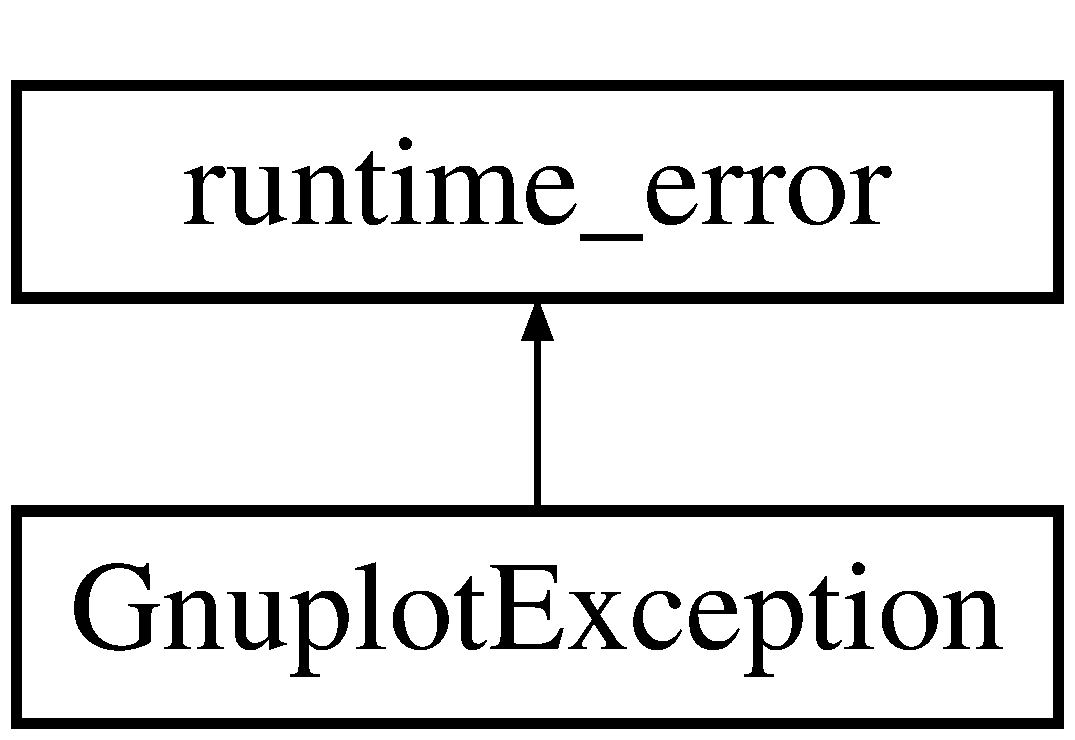
\includegraphics[height=2.000000cm]{class_gnuplot_exception}
\end{center}
\end{figure}
\subsection*{Public Member Functions}
\begin{DoxyCompactItemize}
\item 
\mbox{\Hypertarget{class_gnuplot_exception_a8b324a9ef4d3f75079d41ecd61c62d44}\label{class_gnuplot_exception_a8b324a9ef4d3f75079d41ecd61c62d44}} 
{\bfseries Gnuplot\+Exception} (const std\+::string \&msg)
\end{DoxyCompactItemize}


\subsection{Detailed Description}
A C++ interface to gnuplot. 

The interface uses pipes and so won\textquotesingle{}t run on a system that doesn\textquotesingle{}t have P\+O\+S\+IX pipe support Tested on Windows (Min\+GW and Visual C++) and Linux (G\+CC)

Version history\+: 0. C interface by N. Devillard (27/01/03)
\begin{DoxyEnumerate}
\item C++ interface\+: direct translation from the C interface by Rajarshi Guha (07/03/03)
\item corrections for Win32 compatibility by V. Chyzhdzenka (20/05/03)
\item some member functions added, corrections for Win32 and Linux compatibility by M. Burgis (10/03/08)
\end{DoxyEnumerate}

Requirements\+:
\begin{DoxyItemize}
\item gnuplot has to be installed (\href{http://www.gnuplot.info/download.html}{\tt http\+://www.\+gnuplot.\+info/download.\+html})
\item for Windows\+: set Path-\/\+Variable for \mbox{\hyperlink{class_gnuplot}{Gnuplot}} path (e.\+g. C\+:/program files/gnuplot/bin) or set \mbox{\hyperlink{class_gnuplot}{Gnuplot}} path with\+: \mbox{\hyperlink{class_gnuplot_a67cae885c26ced821e335d98986f1967}{Gnuplot\+::set\+\_\+\+G\+N\+U\+Plot\+Path(const std\+::string \&path)}}; 
\end{DoxyItemize}

The documentation for this class was generated from the following file\+:\begin{DoxyCompactItemize}
\item 
gnuplot\+\_\+i.\+hpp\end{DoxyCompactItemize}

\hypertarget{class_graph___imp}{}\section{Graph\+\_\+\+Imp Class Reference}
\label{class_graph___imp}\index{Graph\+\_\+\+Imp@{Graph\+\_\+\+Imp}}


Defines a class for storing edges of the graph.  




{\ttfamily \#include $<$Graph\+\_\+\+Imp.\+h$>$}

\subsection*{Public Member Functions}
\begin{DoxyCompactItemize}
\item 
\mbox{\Hypertarget{class_graph___imp_a0cc783e97aa1f84bf432c50ecff88472}\label{class_graph___imp_a0cc783e97aa1f84bf432c50ecff88472}} 
\mbox{\hyperlink{class_graph___imp_a0cc783e97aa1f84bf432c50ecff88472}{Graph\+\_\+\+Imp}} ()
\begin{DoxyCompactList}\small\item\em Constructor of class \mbox{\hyperlink{class_graph___imp}{Graph\+\_\+\+Imp}}. \end{DoxyCompactList}\end{DoxyCompactItemize}
\subsection*{Public Attributes}
\begin{DoxyCompactItemize}
\item 
\mbox{\Hypertarget{class_graph___imp_aa361d993a6673de297e714d716ae5159}\label{class_graph___imp_aa361d993a6673de297e714d716ae5159}} 
std\+::vector$<$ \mbox{\hyperlink{struct_triplet}{Triplet}} $>$ \mbox{\hyperlink{class_graph___imp_aa361d993a6673de297e714d716ae5159}{vertices}}
\begin{DoxyCompactList}\small\item\em Vector of \mbox{\hyperlink{struct_triplet}{Triplet}} objects storing all the vertices of the graph. \end{DoxyCompactList}\item 
\mbox{\Hypertarget{class_graph___imp_a294a280b76aaa1b518b7b77c4c717d53}\label{class_graph___imp_a294a280b76aaa1b518b7b77c4c717d53}} 
\mbox{\hyperlink{class_n_graph_1_1t_graph}{N\+Graph\+::\+Graph}} \mbox{\hyperlink{class_graph___imp_a294a280b76aaa1b518b7b77c4c717d53}{edges}}
\begin{DoxyCompactList}\small\item\em \mbox{\hyperlink{namespace_n_graph}{N\+Graph}} object storing all the edges of the graph. \end{DoxyCompactList}\end{DoxyCompactItemize}


\subsection{Detailed Description}
Defines a class for storing edges of the graph. 

Contains the necessary data members and functions required to store edges of the graph 

The documentation for this class was generated from the following file\+:\begin{DoxyCompactItemize}
\item 
Graph\+\_\+\+Imp.\+h\end{DoxyCompactItemize}

\hypertarget{class_show}{}\section{Show Class Reference}
\label{class_show}\index{Show@{Show}}


This is the class which will be used to handle all function related to showing and rendering the graph.  




{\ttfamily \#include $<$Show.\+h$>$}

\subsection*{Public Member Functions}
\begin{DoxyCompactItemize}
\item 
\mbox{\hyperlink{class_graph___imp}{Graph\+\_\+\+Imp}} \mbox{\hyperlink{class_show_ad17a90f324d44a841428434e39e87915}{set\+\_\+acc\+\_\+to\+\_\+ranges}} (\mbox{\hyperlink{class_graph___imp}{Graph\+\_\+\+Imp}} g, int mode)
\begin{DoxyCompactList}\small\item\em Function to scale the graph given to it as an input. \end{DoxyCompactList}\item 
\mbox{\Hypertarget{class_show_a5a1a1552fb8062da10cbc64a16cea844}\label{class_show_a5a1a1552fb8062da10cbc64a16cea844}} 
bool \mbox{\hyperlink{class_show_a5a1a1552fb8062da10cbc64a16cea844}{find\+Edge\+In\+Vector}} (\mbox{\hyperlink{struct_edge}{Edge}} a, std\+::vector$<$ \mbox{\hyperlink{struct_edge}{Edge}} $>$ hidden)
\begin{DoxyCompactList}\small\item\em A function to find an edge in a scaled vector. \end{DoxyCompactList}\item 
void \mbox{\hyperlink{class_show_a0acae4ee3882e2df8671123ea1d7515c}{draw\+Graph}} (\mbox{\hyperlink{class_graph___imp}{Graph\+\_\+\+Imp}} g, Q\+Painter \&p, std\+::vector$<$ \mbox{\hyperlink{struct_edge}{Edge}} $>$ hidden, bool hide)
\begin{DoxyCompactList}\small\item\em Draw the input 2D graph on the Qt\+Canvas. \end{DoxyCompactList}\item 
int \mbox{\hyperlink{class_show_a674f8dc51bcf6c3d5808f5eb411dbf36}{show\+\_\+qt\+\_\+projections}} (\mbox{\hyperlink{class_three___d__to___two___d}{Three\+\_\+\+D\+\_\+to\+\_\+\+Two\+\_\+D}} \&T, \mbox{\hyperlink{struct_triplet}{Triplet}} topdir)
\begin{DoxyCompactList}\small\item\em Main function which takes the 3\+Dto\+TwoD object as an input and makes the projections. \end{DoxyCompactList}\end{DoxyCompactItemize}


\subsection{Detailed Description}
This is the class which will be used to handle all function related to showing and rendering the graph. 

\subsection{Member Function Documentation}
\mbox{\Hypertarget{class_show_a0acae4ee3882e2df8671123ea1d7515c}\label{class_show_a0acae4ee3882e2df8671123ea1d7515c}} 
\index{Show@{Show}!draw\+Graph@{draw\+Graph}}
\index{draw\+Graph@{draw\+Graph}!Show@{Show}}
\subsubsection{\texorpdfstring{draw\+Graph()}{drawGraph()}}
{\footnotesize\ttfamily void Show\+::draw\+Graph (\begin{DoxyParamCaption}\item[{\mbox{\hyperlink{class_graph___imp}{Graph\+\_\+\+Imp}}}]{g,  }\item[{Q\+Painter \&}]{p,  }\item[{std\+::vector$<$ \mbox{\hyperlink{struct_edge}{Edge}} $>$}]{hidden,  }\item[{bool}]{hide }\end{DoxyParamCaption})}



Draw the input 2D graph on the Qt\+Canvas. 


\begin{DoxyParams}{Parameters}
{\em g} & The graph to be shown. \\
\hline
{\em p} & The painter to be used \\
\hline
{\em hidden} & the hidden edges for the current graph. \\
\hline
{\em hide} & Do you want to enable hiding \\
\hline
\end{DoxyParams}
\mbox{\Hypertarget{class_show_ad17a90f324d44a841428434e39e87915}\label{class_show_ad17a90f324d44a841428434e39e87915}} 
\index{Show@{Show}!set\+\_\+acc\+\_\+to\+\_\+ranges@{set\+\_\+acc\+\_\+to\+\_\+ranges}}
\index{set\+\_\+acc\+\_\+to\+\_\+ranges@{set\+\_\+acc\+\_\+to\+\_\+ranges}!Show@{Show}}
\subsubsection{\texorpdfstring{set\+\_\+acc\+\_\+to\+\_\+ranges()}{set\_acc\_to\_ranges()}}
{\footnotesize\ttfamily \mbox{\hyperlink{class_graph___imp}{Graph\+\_\+\+Imp}} Show\+::set\+\_\+acc\+\_\+to\+\_\+ranges (\begin{DoxyParamCaption}\item[{\mbox{\hyperlink{class_graph___imp}{Graph\+\_\+\+Imp}}}]{g,  }\item[{int}]{mode }\end{DoxyParamCaption})}



Function to scale the graph given to it as an input. 


\begin{DoxyParams}{Parameters}
{\em g} & The input graph to be scaled. \\
\hline
{\em mode} & The mode (xy,yz,zx) in which the current scaling has to be done \\
\hline
\end{DoxyParams}
\mbox{\Hypertarget{class_show_a674f8dc51bcf6c3d5808f5eb411dbf36}\label{class_show_a674f8dc51bcf6c3d5808f5eb411dbf36}} 
\index{Show@{Show}!show\+\_\+qt\+\_\+projections@{show\+\_\+qt\+\_\+projections}}
\index{show\+\_\+qt\+\_\+projections@{show\+\_\+qt\+\_\+projections}!Show@{Show}}
\subsubsection{\texorpdfstring{show\+\_\+qt\+\_\+projections()}{show\_qt\_projections()}}
{\footnotesize\ttfamily int Show\+::show\+\_\+qt\+\_\+projections (\begin{DoxyParamCaption}\item[{\mbox{\hyperlink{class_three___d__to___two___d}{Three\+\_\+\+D\+\_\+to\+\_\+\+Two\+\_\+D}} \&}]{T,  }\item[{\mbox{\hyperlink{struct_triplet}{Triplet}}}]{topdir }\end{DoxyParamCaption})}



Main function which takes the 3\+Dto\+TwoD object as an input and makes the projections. 

/param T The object to be projected /param topdir The direction ratios for rotation 

The documentation for this class was generated from the following file\+:\begin{DoxyCompactItemize}
\item 
Show.\+h\end{DoxyCompactItemize}

\hypertarget{class_n_graph_1_1t_graph}{}\section{N\+Graph\+:\+:t\+Graph$<$ T $>$ Class Template Reference}
\label{class_n_graph_1_1t_graph}\index{N\+Graph\+::t\+Graph$<$ T $>$@{N\+Graph\+::t\+Graph$<$ T $>$}}
\subsection*{Public Types}
\begin{DoxyCompactItemize}
\item 
\mbox{\Hypertarget{class_n_graph_1_1t_graph_a4a14eff6bcee7d8c0528c13d5e99ad71}\label{class_n_graph_1_1t_graph_a4a14eff6bcee7d8c0528c13d5e99ad71}} 
enum {\bfseries line\+\_\+type} \{ {\bfseries V\+E\+R\+T\+EX}, 
{\bfseries E\+D\+GE}, 
{\bfseries C\+O\+M\+M\+E\+NT}, 
{\bfseries E\+M\+P\+TY}
 \}
\item 
\mbox{\Hypertarget{class_n_graph_1_1t_graph_a63a04bf8bfc7cf968be524208f49fdee}\label{class_n_graph_1_1t_graph_a63a04bf8bfc7cf968be524208f49fdee}} 
typedef T {\bfseries vertex}
\item 
\mbox{\Hypertarget{class_n_graph_1_1t_graph_addb8e5aa5779f80e19e368eef9448e8c}\label{class_n_graph_1_1t_graph_addb8e5aa5779f80e19e368eef9448e8c}} 
typedef T {\bfseries value\+\_\+type}
\item 
\mbox{\Hypertarget{class_n_graph_1_1t_graph_a6c85cd9c55a19c3c052f176fe719fdfc}\label{class_n_graph_1_1t_graph_a6c85cd9c55a19c3c052f176fe719fdfc}} 
typedef std\+::pair$<$ vertex, vertex $>$ {\bfseries edge}
\item 
\mbox{\Hypertarget{class_n_graph_1_1t_graph_a9e0a5df1ac9a2e6df94431aeaf610b3e}\label{class_n_graph_1_1t_graph_a9e0a5df1ac9a2e6df94431aeaf610b3e}} 
typedef std\+::set$<$ vertex $>$ {\bfseries vertex\+\_\+set}
\item 
\mbox{\Hypertarget{class_n_graph_1_1t_graph_a18a0c72c7ef57d877cab05bba5cf4d9b}\label{class_n_graph_1_1t_graph_a18a0c72c7ef57d877cab05bba5cf4d9b}} 
typedef std\+::set$<$ edge $>$ {\bfseries edge\+\_\+set}
\item 
\mbox{\Hypertarget{class_n_graph_1_1t_graph_a9822c284aa101d90d3bd613c7e05eaa4}\label{class_n_graph_1_1t_graph_a9822c284aa101d90d3bd613c7e05eaa4}} 
typedef std\+::pair$<$ vertex\+\_\+set, vertex\+\_\+set $>$ {\bfseries in\+\_\+out\+\_\+edge\+\_\+sets}
\item 
\mbox{\Hypertarget{class_n_graph_1_1t_graph_a0036686b7a2d33d0c2aeca3f6715495d}\label{class_n_graph_1_1t_graph_a0036686b7a2d33d0c2aeca3f6715495d}} 
typedef std\+::map$<$ vertex, in\+\_\+out\+\_\+edge\+\_\+sets $>$ {\bfseries adj\+\_\+graph}
\item 
\mbox{\Hypertarget{class_n_graph_1_1t_graph_a1b710c759e101724f3544b374ebb0179}\label{class_n_graph_1_1t_graph_a1b710c759e101724f3544b374ebb0179}} 
typedef edge\+\_\+set\+::iterator {\bfseries edge\+\_\+iterator}
\item 
\mbox{\Hypertarget{class_n_graph_1_1t_graph_a6e189d2dd98fbe980b830d898eea5247}\label{class_n_graph_1_1t_graph_a6e189d2dd98fbe980b830d898eea5247}} 
typedef edge\+\_\+set\+::const\+\_\+iterator {\bfseries const\+\_\+edge\+\_\+iterator}
\item 
\mbox{\Hypertarget{class_n_graph_1_1t_graph_ad5c343cc3c50b291b35fb48147db3250}\label{class_n_graph_1_1t_graph_ad5c343cc3c50b291b35fb48147db3250}} 
typedef vertex\+\_\+set\+::iterator {\bfseries vertex\+\_\+iterator}
\item 
\mbox{\Hypertarget{class_n_graph_1_1t_graph_a5ed9ca8ad9676b3c7abd3880f735ce80}\label{class_n_graph_1_1t_graph_a5ed9ca8ad9676b3c7abd3880f735ce80}} 
typedef vertex\+\_\+set\+::const\+\_\+iterator {\bfseries const\+\_\+vertex\+\_\+iterator}
\item 
\mbox{\Hypertarget{class_n_graph_1_1t_graph_aeb3fd2cc092aa7ecb4b749ee4e78f9ab}\label{class_n_graph_1_1t_graph_aeb3fd2cc092aa7ecb4b749ee4e78f9ab}} 
typedef vertex\+\_\+set\+::iterator {\bfseries vertex\+\_\+neighbor\+\_\+iterator}
\item 
\mbox{\Hypertarget{class_n_graph_1_1t_graph_af8b0bc7076b28fb145b267b8faad195e}\label{class_n_graph_1_1t_graph_af8b0bc7076b28fb145b267b8faad195e}} 
typedef vertex\+\_\+set\+::const\+\_\+iterator {\bfseries vertex\+\_\+neighbor\+\_\+const\+\_\+iterator}
\item 
typedef adj\+\_\+graph\+::iterator \mbox{\hyperlink{class_n_graph_1_1t_graph_a6e446a33b74e5c0c39fb6c50a4f07cec}{iterator}}
\item 
\mbox{\Hypertarget{class_n_graph_1_1t_graph_a64864813622245ff9412c784232f2f99}\label{class_n_graph_1_1t_graph_a64864813622245ff9412c784232f2f99}} 
typedef adj\+\_\+graph\+::const\+\_\+iterator {\bfseries const\+\_\+iterator}
\item 
\mbox{\Hypertarget{class_n_graph_1_1t_graph_af9638aed082c5e33cf4064f158f66d59}\label{class_n_graph_1_1t_graph_af9638aed082c5e33cf4064f158f66d59}} 
typedef \mbox{\hyperlink{class_n_graph_1_1t_graph_a6e446a33b74e5c0c39fb6c50a4f07cec}{iterator}} {\bfseries node\+\_\+iterator}
\item 
\mbox{\Hypertarget{class_n_graph_1_1t_graph_a4a4c169ed8eecce822b2d18b21082ce7}\label{class_n_graph_1_1t_graph_a4a4c169ed8eecce822b2d18b21082ce7}} 
typedef const\+\_\+iterator {\bfseries const\+\_\+node\+\_\+iterator}
\end{DoxyCompactItemize}
\subsection*{Public Member Functions}
\begin{DoxyCompactItemize}
\item 
\mbox{\Hypertarget{class_n_graph_1_1t_graph_a6aff4cfa2819f372ce4c7030c9709b82}\label{class_n_graph_1_1t_graph_a6aff4cfa2819f372ce4c7030c9709b82}} 
unsigned int {\bfseries num\+\_\+vertices} () const
\item 
\mbox{\Hypertarget{class_n_graph_1_1t_graph_a5bbc421c6e9181fbd42ca1255b6fa739}\label{class_n_graph_1_1t_graph_a5bbc421c6e9181fbd42ca1255b6fa739}} 
unsigned int {\bfseries num\+\_\+nodes} () const
\item 
\mbox{\Hypertarget{class_n_graph_1_1t_graph_a25a5ca5600c3c4d4ae58f945981b5561}\label{class_n_graph_1_1t_graph_a25a5ca5600c3c4d4ae58f945981b5561}} 
unsigned int {\bfseries num\+\_\+edges} () const
\item 
\mbox{\Hypertarget{class_n_graph_1_1t_graph_a1fa503849355f65f3d235b895a3f6086}\label{class_n_graph_1_1t_graph_a1fa503849355f65f3d235b895a3f6086}} 
\mbox{\hyperlink{class_n_graph_1_1t_graph_a6e446a33b74e5c0c39fb6c50a4f07cec}{iterator}} {\bfseries begin} ()
\item 
\mbox{\Hypertarget{class_n_graph_1_1t_graph_a957235ebde0cfda1bdfacdd0db212d73}\label{class_n_graph_1_1t_graph_a957235ebde0cfda1bdfacdd0db212d73}} 
const\+\_\+iterator {\bfseries begin} () const
\item 
\mbox{\Hypertarget{class_n_graph_1_1t_graph_a78775c7c87001e8ceb5668cec6d40dfb}\label{class_n_graph_1_1t_graph_a78775c7c87001e8ceb5668cec6d40dfb}} 
\mbox{\hyperlink{class_n_graph_1_1t_graph_a6e446a33b74e5c0c39fb6c50a4f07cec}{iterator}} {\bfseries end} ()
\item 
\mbox{\Hypertarget{class_n_graph_1_1t_graph_aca77137373df2e5313f434326ffc355a}\label{class_n_graph_1_1t_graph_aca77137373df2e5313f434326ffc355a}} 
const\+\_\+iterator {\bfseries end} () const
\item 
\mbox{\Hypertarget{class_n_graph_1_1t_graph_add822443b93ee9ef745ee3b8ab12065b}\label{class_n_graph_1_1t_graph_add822443b93ee9ef745ee3b8ab12065b}} 
void {\bfseries clear} ()
\item 
\mbox{\Hypertarget{class_n_graph_1_1t_graph_af4aaf8e70f041bea0759caa9133f5fe6}\label{class_n_graph_1_1t_graph_af4aaf8e70f041bea0759caa9133f5fe6}} 
vertex\+\_\+neighbor\+\_\+iterator {\bfseries out\+\_\+neighbors\+\_\+begin} (const vertex \&a)
\item 
\mbox{\Hypertarget{class_n_graph_1_1t_graph_a58a0b9135d7fdc9bd9bccb37f477ea12}\label{class_n_graph_1_1t_graph_a58a0b9135d7fdc9bd9bccb37f477ea12}} 
vertex\+\_\+neighbor\+\_\+const\+\_\+iterator {\bfseries out\+\_\+neighbors\+\_\+begin} (const vertex \&a) const
\item 
\mbox{\Hypertarget{class_n_graph_1_1t_graph_a85890eeb0085d0079824acc5a8c0240b}\label{class_n_graph_1_1t_graph_a85890eeb0085d0079824acc5a8c0240b}} 
vertex\+\_\+neighbor\+\_\+iterator {\bfseries out\+\_\+neighbors\+\_\+end} (const vertex \&a)
\item 
\mbox{\Hypertarget{class_n_graph_1_1t_graph_a90ed49e6b1a6b555713370d8cc3a11c9}\label{class_n_graph_1_1t_graph_a90ed49e6b1a6b555713370d8cc3a11c9}} 
vertex\+\_\+neighbor\+\_\+const\+\_\+iterator {\bfseries out\+\_\+neighbors\+\_\+end} (const vertex \&a) const
\item 
\mbox{\Hypertarget{class_n_graph_1_1t_graph_a548e93259bcece749bed2d6375049be9}\label{class_n_graph_1_1t_graph_a548e93259bcece749bed2d6375049be9}} 
{\bfseries t\+Graph} (std\+::istream \&s)
\item 
\mbox{\Hypertarget{class_n_graph_1_1t_graph_a70928f9e49923184ee26a228ebd23ff5}\label{class_n_graph_1_1t_graph_a70928f9e49923184ee26a228ebd23ff5}} 
{\bfseries t\+Graph} (const \mbox{\hyperlink{class_n_graph_1_1t_graph}{t\+Graph}} \&B)
\item 
\mbox{\Hypertarget{class_n_graph_1_1t_graph_a8267a8db43eae2dd34d1d50db57e821c}\label{class_n_graph_1_1t_graph_a8267a8db43eae2dd34d1d50db57e821c}} 
{\bfseries t\+Graph} (const edge\+\_\+set \&E)
\item 
\mbox{\Hypertarget{class_n_graph_1_1t_graph_a512ce90c67d43855c0f6b131a90dfbce}\label{class_n_graph_1_1t_graph_a512ce90c67d43855c0f6b131a90dfbce}} 
bool {\bfseries is\+\_\+undirected} () const
\item 
\mbox{\Hypertarget{class_n_graph_1_1t_graph_a0533e8f86aceaa221f64d835178fd966}\label{class_n_graph_1_1t_graph_a0533e8f86aceaa221f64d835178fd966}} 
bool {\bfseries is\+\_\+directed} () const
\item 
\mbox{\Hypertarget{class_n_graph_1_1t_graph_a374bc267c08ca80f7bece5f2230848d0}\label{class_n_graph_1_1t_graph_a374bc267c08ca80f7bece5f2230848d0}} 
void {\bfseries set\+\_\+undirected} ()
\item 
\mbox{\Hypertarget{class_n_graph_1_1t_graph_a94305809ed5bd6531d73e74d5b63055f}\label{class_n_graph_1_1t_graph_a94305809ed5bd6531d73e74d5b63055f}} 
\mbox{\hyperlink{class_n_graph_1_1t_graph_a6e446a33b74e5c0c39fb6c50a4f07cec}{iterator}} {\bfseries find} (const vertex \&a)
\item 
\mbox{\Hypertarget{class_n_graph_1_1t_graph_a15801328dc81c8eff05ce09dd4094b28}\label{class_n_graph_1_1t_graph_a15801328dc81c8eff05ce09dd4094b28}} 
const\+\_\+iterator {\bfseries find} (const vertex \&a) const
\item 
\mbox{\Hypertarget{class_n_graph_1_1t_graph_a58f5d07e8dfe45d237d093c5bc11ad53}\label{class_n_graph_1_1t_graph_a58f5d07e8dfe45d237d093c5bc11ad53}} 
const vertex\+\_\+set \& {\bfseries in\+\_\+neighbors} (const vertex \&a) const
\item 
\mbox{\Hypertarget{class_n_graph_1_1t_graph_a0ca32078d83236c669a6e0beb7d93759}\label{class_n_graph_1_1t_graph_a0ca32078d83236c669a6e0beb7d93759}} 
vertex\+\_\+set \& {\bfseries in\+\_\+neighbors} (const vertex \&a)
\item 
\mbox{\Hypertarget{class_n_graph_1_1t_graph_acffca17cd25301de3d6aa8a132c4431f}\label{class_n_graph_1_1t_graph_acffca17cd25301de3d6aa8a132c4431f}} 
const vertex\+\_\+set \& {\bfseries out\+\_\+neighbors} (const vertex \&a) const
\item 
\mbox{\Hypertarget{class_n_graph_1_1t_graph_acb50f260b7b391b7c6a73a640bacc08d}\label{class_n_graph_1_1t_graph_acb50f260b7b391b7c6a73a640bacc08d}} 
vertex\+\_\+set \& {\bfseries out\+\_\+neighbors} (const vertex \&a)
\item 
\mbox{\Hypertarget{class_n_graph_1_1t_graph_a1e6a83e13c11c16599567f6d50e658c2}\label{class_n_graph_1_1t_graph_a1e6a83e13c11c16599567f6d50e658c2}} 
unsigned int {\bfseries in\+\_\+degree} (const vertex \&a) const
\item 
\mbox{\Hypertarget{class_n_graph_1_1t_graph_afa6b411ff31557d044b02f87bbe50999}\label{class_n_graph_1_1t_graph_afa6b411ff31557d044b02f87bbe50999}} 
unsigned int {\bfseries out\+\_\+degree} (const vertex \&a) const
\item 
\mbox{\Hypertarget{class_n_graph_1_1t_graph_a717a15800fec8ebefde8d2d853390a0b}\label{class_n_graph_1_1t_graph_a717a15800fec8ebefde8d2d853390a0b}} 
unsigned int {\bfseries degree} (const vertex \&a) const
\item 
\mbox{\Hypertarget{class_n_graph_1_1t_graph_a0352a3bfc0fc6d2ce59395d1f0064550}\label{class_n_graph_1_1t_graph_a0352a3bfc0fc6d2ce59395d1f0064550}} 
bool {\bfseries isolated} (const vertex \&a) const
\item 
\mbox{\Hypertarget{class_n_graph_1_1t_graph_ae7e728e1249dc0fcb4e2ebec1e4ae6dd}\label{class_n_graph_1_1t_graph_ae7e728e1249dc0fcb4e2ebec1e4ae6dd}} 
void {\bfseries insert\+\_\+vertex} (const vertex \&a)
\item 
\mbox{\Hypertarget{class_n_graph_1_1t_graph_a5fb33cf26902838865ac86fc51123a96}\label{class_n_graph_1_1t_graph_a5fb33cf26902838865ac86fc51123a96}} 
void {\bfseries insert\+\_\+new\+\_\+vertex\+\_\+inout\+\_\+list} (const vertex \&a, const vertex\+\_\+set \&IN, const vertex\+\_\+set \&O\+UT)
\item 
\mbox{\Hypertarget{class_n_graph_1_1t_graph_a3227d649839908a87afbd80316cc493f}\label{class_n_graph_1_1t_graph_a3227d649839908a87afbd80316cc493f}} 
void {\bfseries insert\+\_\+edge\+\_\+noloop} (\mbox{\hyperlink{class_n_graph_1_1t_graph_a6e446a33b74e5c0c39fb6c50a4f07cec}{iterator}} pa, \mbox{\hyperlink{class_n_graph_1_1t_graph_a6e446a33b74e5c0c39fb6c50a4f07cec}{iterator}} pb)
\item 
\mbox{\Hypertarget{class_n_graph_1_1t_graph_a5ee540bb69a2bdd199b63af489439545}\label{class_n_graph_1_1t_graph_a5ee540bb69a2bdd199b63af489439545}} 
void {\bfseries insert\+\_\+edge} (\mbox{\hyperlink{class_n_graph_1_1t_graph_a6e446a33b74e5c0c39fb6c50a4f07cec}{iterator}} pa, \mbox{\hyperlink{class_n_graph_1_1t_graph_a6e446a33b74e5c0c39fb6c50a4f07cec}{iterator}} pb)
\item 
\mbox{\Hypertarget{class_n_graph_1_1t_graph_ad8ef6d934af47685338257274e421bab}\label{class_n_graph_1_1t_graph_ad8ef6d934af47685338257274e421bab}} 
void {\bfseries insert\+\_\+edge\+\_\+noloop} (const vertex \&a, const vertex \&b)
\item 
\mbox{\Hypertarget{class_n_graph_1_1t_graph_a7e62b364e0a03fb416facee8b51d99da}\label{class_n_graph_1_1t_graph_a7e62b364e0a03fb416facee8b51d99da}} 
void {\bfseries insert\+\_\+edge} (const vertex \&a, const vertex \&b)
\item 
\mbox{\Hypertarget{class_n_graph_1_1t_graph_a6a0b8b06f321534275d982ae500a4df3}\label{class_n_graph_1_1t_graph_a6a0b8b06f321534275d982ae500a4df3}} 
void {\bfseries insert\+\_\+undirected\+\_\+edge} (const vertex \&a, const vertex \&b)
\item 
\mbox{\Hypertarget{class_n_graph_1_1t_graph_a7aa85e0fe919a7c6fafac8051271421b}\label{class_n_graph_1_1t_graph_a7aa85e0fe919a7c6fafac8051271421b}} 
void {\bfseries insert\+\_\+edge} (const edge \&E)
\item 
\mbox{\Hypertarget{class_n_graph_1_1t_graph_a90d80d85d509b09c932fde138fb0aae0}\label{class_n_graph_1_1t_graph_a90d80d85d509b09c932fde138fb0aae0}} 
void {\bfseries insert\+\_\+undirected\+\_\+edge} (const edge \&E)
\item 
\mbox{\Hypertarget{class_n_graph_1_1t_graph_a5af6f7dbadd1f355987bca99d210ebdb}\label{class_n_graph_1_1t_graph_a5af6f7dbadd1f355987bca99d210ebdb}} 
bool {\bfseries remove\+\_\+edge} (\mbox{\hyperlink{class_n_graph_1_1t_graph_a6e446a33b74e5c0c39fb6c50a4f07cec}{iterator}} pa, \mbox{\hyperlink{class_n_graph_1_1t_graph_a6e446a33b74e5c0c39fb6c50a4f07cec}{iterator}} pb)
\item 
\mbox{\Hypertarget{class_n_graph_1_1t_graph_ac1fff890e65f3f1654a79a8574b13378}\label{class_n_graph_1_1t_graph_ac1fff890e65f3f1654a79a8574b13378}} 
void {\bfseries remove\+\_\+edge} (const vertex \&a, const vertex \&b)
\item 
\mbox{\Hypertarget{class_n_graph_1_1t_graph_ac64968018b02ebd689cb9acb96409327}\label{class_n_graph_1_1t_graph_ac64968018b02ebd689cb9acb96409327}} 
void {\bfseries remove\+\_\+edge} (const edge \&E)
\item 
\mbox{\Hypertarget{class_n_graph_1_1t_graph_af18958f28aaa6be4aa3ba3e273e5dae3}\label{class_n_graph_1_1t_graph_af18958f28aaa6be4aa3ba3e273e5dae3}} 
void {\bfseries remove\+\_\+undirected\+\_\+edge} (const vertex \&a, const vertex \&b)
\item 
\mbox{\Hypertarget{class_n_graph_1_1t_graph_aa4d5dc7efdb07adb6de626f625701478}\label{class_n_graph_1_1t_graph_aa4d5dc7efdb07adb6de626f625701478}} 
void {\bfseries remove\+\_\+undirected\+\_\+edge} (const edge \&e)
\item 
\mbox{\Hypertarget{class_n_graph_1_1t_graph_ae3ddcc68cfd75c8a8c11a47fc1a449b9}\label{class_n_graph_1_1t_graph_ae3ddcc68cfd75c8a8c11a47fc1a449b9}} 
void {\bfseries remove\+\_\+vertex} (\mbox{\hyperlink{class_n_graph_1_1t_graph_a6e446a33b74e5c0c39fb6c50a4f07cec}{iterator}} pa)
\item 
\mbox{\Hypertarget{class_n_graph_1_1t_graph_adfdabb4a748158e58d1a19ed1ef4fdf1}\label{class_n_graph_1_1t_graph_adfdabb4a748158e58d1a19ed1ef4fdf1}} 
void {\bfseries remove\+\_\+vertex\+\_\+set} (const vertex\+\_\+set \&V)
\item 
\mbox{\Hypertarget{class_n_graph_1_1t_graph_a33aa30bb79f01806408465f1250cac0d}\label{class_n_graph_1_1t_graph_a33aa30bb79f01806408465f1250cac0d}} 
void {\bfseries remove\+\_\+vertex} (const vertex \&a)
\item 
bool \mbox{\hyperlink{class_n_graph_1_1t_graph_a260849918a2806a4a9aa1cfad0471e41}{includes\+\_\+vertex}} (const vertex \&a) const
\item 
bool \mbox{\hyperlink{class_n_graph_1_1t_graph_a463b923ee1e3604407837150f17f1a74}{includes\+\_\+edge}} (const vertex \&a, const vertex \&b) const
\item 
\mbox{\Hypertarget{class_n_graph_1_1t_graph_a8d364cdfbd44f0804a91bdcda683b31b}\label{class_n_graph_1_1t_graph_a8d364cdfbd44f0804a91bdcda683b31b}} 
bool {\bfseries includes\+\_\+edge} (const edge \&e) const
\item 
std\+::vector$<$ edge $>$ \mbox{\hyperlink{class_n_graph_1_1t_graph_a4f7e150eadbb8845e8f858255022a037}{edge\+\_\+list}} () const
\item 
\mbox{\Hypertarget{class_n_graph_1_1t_graph_af5ad33beb237d62d6a36e1559f50bce1}\label{class_n_graph_1_1t_graph_af5ad33beb237d62d6a36e1559f50bce1}} 
\mbox{\hyperlink{class_n_graph_1_1t_graph}{t\+Graph}} \& {\bfseries plus\+\_\+eq} (const \mbox{\hyperlink{class_n_graph_1_1t_graph}{t\+Graph}} \&B)
\item 
\mbox{\Hypertarget{class_n_graph_1_1t_graph_ac2ddbf2173c45a06dbccece30cacb98f}\label{class_n_graph_1_1t_graph_ac2ddbf2173c45a06dbccece30cacb98f}} 
\mbox{\hyperlink{class_n_graph_1_1t_graph}{t\+Graph}} {\bfseries intersect} (const \mbox{\hyperlink{class_n_graph_1_1t_graph}{t\+Graph}} \&B) const
\item 
\mbox{\Hypertarget{class_n_graph_1_1t_graph_ad899ac4d991eae39c7cd1d8a7b424ac0}\label{class_n_graph_1_1t_graph_ad899ac4d991eae39c7cd1d8a7b424ac0}} 
\mbox{\hyperlink{class_n_graph_1_1t_graph}{t\+Graph}} {\bfseries operator$\ast$} (const \mbox{\hyperlink{class_n_graph_1_1t_graph}{t\+Graph}} \&B) const
\item 
\mbox{\Hypertarget{class_n_graph_1_1t_graph_a7b00a9cf016faa75da9dcc429fe503d3}\label{class_n_graph_1_1t_graph_a7b00a9cf016faa75da9dcc429fe503d3}} 
\mbox{\hyperlink{class_n_graph_1_1t_graph}{t\+Graph}} {\bfseries minus} (const \mbox{\hyperlink{class_n_graph_1_1t_graph}{t\+Graph}} \&B) const
\item 
\mbox{\Hypertarget{class_n_graph_1_1t_graph_ae09dcf65e16d50b26515716ec52fb71f}\label{class_n_graph_1_1t_graph_ae09dcf65e16d50b26515716ec52fb71f}} 
\mbox{\hyperlink{class_n_graph_1_1t_graph}{t\+Graph}} {\bfseries operator-\/} (const \mbox{\hyperlink{class_n_graph_1_1t_graph}{t\+Graph}} \&B) const
\item 
\mbox{\Hypertarget{class_n_graph_1_1t_graph_ab9d3103f422170bce7c7a2c952c56024}\label{class_n_graph_1_1t_graph_ab9d3103f422170bce7c7a2c952c56024}} 
\mbox{\hyperlink{class_n_graph_1_1t_graph}{t\+Graph}} {\bfseries plus} (const \mbox{\hyperlink{class_n_graph_1_1t_graph}{t\+Graph}} \&B) const
\item 
\mbox{\Hypertarget{class_n_graph_1_1t_graph_aceb173f4fd1cfb252a33d978c62ff49f}\label{class_n_graph_1_1t_graph_aceb173f4fd1cfb252a33d978c62ff49f}} 
\mbox{\hyperlink{class_n_graph_1_1t_graph}{t\+Graph}} {\bfseries operator+} (const \mbox{\hyperlink{class_n_graph_1_1t_graph}{t\+Graph}} \&B) const
\item 
\mbox{\Hypertarget{class_n_graph_1_1t_graph_a329c3e80609a8bf3c2f6e00ab8298e3d}\label{class_n_graph_1_1t_graph_a329c3e80609a8bf3c2f6e00ab8298e3d}} 
\mbox{\hyperlink{class_n_graph_1_1t_graph}{t\+Graph}} \& {\bfseries operator+=} (const \mbox{\hyperlink{class_n_graph_1_1t_graph}{t\+Graph}} \&B)
\item 
\mbox{\hyperlink{class_n_graph_1_1t_graph}{t\+Graph}} \mbox{\hyperlink{class_n_graph_1_1t_graph_ab685e653704db79f06216d0d5977f153}{subgraph}} (const vertex\+\_\+set \&A) const
\item 
\mbox{\Hypertarget{class_n_graph_1_1t_graph_ae8f6d218e22f2271aab306e10c252201}\label{class_n_graph_1_1t_graph_ae8f6d218e22f2271aab306e10c252201}} 
unsigned int {\bfseries subgraph\+\_\+size} (const vertex\+\_\+set \&A) const
\item 
\mbox{\Hypertarget{class_n_graph_1_1t_graph_a99c4a072f1445173ca8f36b711f60954}\label{class_n_graph_1_1t_graph_a99c4a072f1445173ca8f36b711f60954}} 
double {\bfseries subgraph\+\_\+sparsity} (const vertex\+\_\+set \&A) const
\item 
\mbox{\Hypertarget{class_n_graph_1_1t_graph_aa9a8cb7d229675823a308ab361b849e2}\label{class_n_graph_1_1t_graph_aa9a8cb7d229675823a308ab361b849e2}} 
void {\bfseries print} () const
\item 
void \mbox{\hyperlink{class_n_graph_1_1t_graph_a1844ff9c48370c79147c84384f400c80}{absorb}} (\mbox{\hyperlink{class_n_graph_1_1t_graph_a6e446a33b74e5c0c39fb6c50a4f07cec}{iterator}} pa, \mbox{\hyperlink{class_n_graph_1_1t_graph_a6e446a33b74e5c0c39fb6c50a4f07cec}{iterator}} pb)
\item 
\mbox{\hyperlink{class_n_graph_1_1t_graph_a6e446a33b74e5c0c39fb6c50a4f07cec}{iterator}} \mbox{\hyperlink{class_n_graph_1_1t_graph_aa3752935ebcd6e4688b52cd0f6d1211f}{smart\+\_\+absorb}} (\mbox{\hyperlink{class_n_graph_1_1t_graph_a6e446a33b74e5c0c39fb6c50a4f07cec}{iterator}} pa, \mbox{\hyperlink{class_n_graph_1_1t_graph_a6e446a33b74e5c0c39fb6c50a4f07cec}{iterator}} pb)
\item 
\mbox{\Hypertarget{class_n_graph_1_1t_graph_a35015ce8e51b4301e69d542c21d26c46}\label{class_n_graph_1_1t_graph_a35015ce8e51b4301e69d542c21d26c46}} 
vertex {\bfseries smart\+\_\+absorb} (vertex a, vertex b)
\item 
\mbox{\Hypertarget{class_n_graph_1_1t_graph_ace64fe566c1df5b77770b4f3ff9ceca0}\label{class_n_graph_1_1t_graph_ace64fe566c1df5b77770b4f3ff9ceca0}} 
void {\bfseries absorb} (vertex a, vertex b)
\end{DoxyCompactItemize}
\subsection*{Static Public Member Functions}
\begin{DoxyCompactItemize}
\item 
static const vertex \& \mbox{\hyperlink{class_n_graph_1_1t_graph_a826e79cbe8d540de7f044c6ae841dd5f}{node}} (const\+\_\+iterator p)
\item 
\mbox{\Hypertarget{class_n_graph_1_1t_graph_a2f6c033bad7dd6e4883de81510901aec}\label{class_n_graph_1_1t_graph_a2f6c033bad7dd6e4883de81510901aec}} 
static const vertex \& {\bfseries node} (\mbox{\hyperlink{class_n_graph_1_1t_graph_a6e446a33b74e5c0c39fb6c50a4f07cec}{iterator}} p)
\item 
\mbox{\Hypertarget{class_n_graph_1_1t_graph_a4bc654a0d0ddba8df6048e4eac5a1729}\label{class_n_graph_1_1t_graph_a4bc654a0d0ddba8df6048e4eac5a1729}} 
static const vertex \& {\bfseries node} (const\+\_\+vertex\+\_\+iterator p)
\item 
\mbox{\Hypertarget{class_n_graph_1_1t_graph_a820f6a863d8d838cd4403b9156bc959a}\label{class_n_graph_1_1t_graph_a820f6a863d8d838cd4403b9156bc959a}} 
static const vertex\+\_\+set \& {\bfseries in\+\_\+neighbors} (const\+\_\+iterator p)
\item 
\mbox{\Hypertarget{class_n_graph_1_1t_graph_aca61e35bcd5af8b66b3c87673771508d}\label{class_n_graph_1_1t_graph_aca61e35bcd5af8b66b3c87673771508d}} 
static vertex\+\_\+set \& {\bfseries in\+\_\+neighbors} (\mbox{\hyperlink{class_n_graph_1_1t_graph_a6e446a33b74e5c0c39fb6c50a4f07cec}{iterator}} p)
\item 
\mbox{\Hypertarget{class_n_graph_1_1t_graph_a3152b5d0315b94d8cb1b24a70988d990}\label{class_n_graph_1_1t_graph_a3152b5d0315b94d8cb1b24a70988d990}} 
static const\+\_\+vertex\+\_\+iterator {\bfseries in\+\_\+begin} (const\+\_\+iterator p)
\item 
\mbox{\Hypertarget{class_n_graph_1_1t_graph_a89d7cf140e48b1d37b6534035872ab88}\label{class_n_graph_1_1t_graph_a89d7cf140e48b1d37b6534035872ab88}} 
static const\+\_\+vertex\+\_\+iterator {\bfseries in\+\_\+end} (const\+\_\+iterator p)
\item 
\mbox{\Hypertarget{class_n_graph_1_1t_graph_a1bd0815f5c00d624dbed8bddffab19ae}\label{class_n_graph_1_1t_graph_a1bd0815f5c00d624dbed8bddffab19ae}} 
static const vertex\+\_\+set \& {\bfseries out\+\_\+neighbors} (const\+\_\+iterator p)
\item 
\mbox{\Hypertarget{class_n_graph_1_1t_graph_a43c8b50d4a2a21c5e673510e76fa303e}\label{class_n_graph_1_1t_graph_a43c8b50d4a2a21c5e673510e76fa303e}} 
static const\+\_\+vertex\+\_\+iterator {\bfseries out\+\_\+begin} (const\+\_\+iterator p)
\item 
\mbox{\Hypertarget{class_n_graph_1_1t_graph_af485a8c7b28e7aa81fbc7cf65316dc21}\label{class_n_graph_1_1t_graph_af485a8c7b28e7aa81fbc7cf65316dc21}} 
static const\+\_\+vertex\+\_\+iterator {\bfseries out\+\_\+end} (const\+\_\+iterator p)
\item 
\mbox{\Hypertarget{class_n_graph_1_1t_graph_aab1fb0576d1eb5604779bf0f7ad6d60d}\label{class_n_graph_1_1t_graph_aab1fb0576d1eb5604779bf0f7ad6d60d}} 
static vertex\+\_\+set \& {\bfseries out\+\_\+neighbors} (\mbox{\hyperlink{class_n_graph_1_1t_graph_a6e446a33b74e5c0c39fb6c50a4f07cec}{iterator}} p)
\item 
\mbox{\Hypertarget{class_n_graph_1_1t_graph_a8c782dadf12b75e66f8db04c60763cbe}\label{class_n_graph_1_1t_graph_a8c782dadf12b75e66f8db04c60763cbe}} 
static vertex\+\_\+iterator {\bfseries out\+\_\+begin} (\mbox{\hyperlink{class_n_graph_1_1t_graph_a6e446a33b74e5c0c39fb6c50a4f07cec}{iterator}} p)
\item 
\mbox{\Hypertarget{class_n_graph_1_1t_graph_a1a850ec5708546dfca02d8a78d41a878}\label{class_n_graph_1_1t_graph_a1a850ec5708546dfca02d8a78d41a878}} 
static unsigned int {\bfseries num\+\_\+edges} (const\+\_\+iterator p)
\item 
\mbox{\Hypertarget{class_n_graph_1_1t_graph_a988ba97d4db2eaa9d9e0ef28658f0d8d}\label{class_n_graph_1_1t_graph_a988ba97d4db2eaa9d9e0ef28658f0d8d}} 
static unsigned int {\bfseries num\+\_\+edges} (\mbox{\hyperlink{class_n_graph_1_1t_graph_a6e446a33b74e5c0c39fb6c50a4f07cec}{iterator}} p)
\item 
static unsigned int \mbox{\hyperlink{class_n_graph_1_1t_graph_acd67259b93d9ec2de6ca03bf19e027bd}{out\+\_\+degree}} (const\+\_\+iterator p)
\item 
\mbox{\Hypertarget{class_n_graph_1_1t_graph_a855dcfd91171425d09a60593bd222a2b}\label{class_n_graph_1_1t_graph_a855dcfd91171425d09a60593bd222a2b}} 
static unsigned int {\bfseries out\+\_\+degree} (\mbox{\hyperlink{class_n_graph_1_1t_graph_a6e446a33b74e5c0c39fb6c50a4f07cec}{iterator}} p)
\item 
static unsigned int \mbox{\hyperlink{class_n_graph_1_1t_graph_a5c269fb5cb63c82496bb9c59d6c289b1}{in\+\_\+degree}} (const\+\_\+iterator p)
\item 
\mbox{\Hypertarget{class_n_graph_1_1t_graph_addc7a2aa0c3aa9b2c21cf50b27ec0d63}\label{class_n_graph_1_1t_graph_addc7a2aa0c3aa9b2c21cf50b27ec0d63}} 
static unsigned int {\bfseries in\+\_\+degree} (\mbox{\hyperlink{class_n_graph_1_1t_graph_a6e446a33b74e5c0c39fb6c50a4f07cec}{iterator}} p)
\item 
\mbox{\Hypertarget{class_n_graph_1_1t_graph_a22f2c477b95c7a7bbf4ad117f1905d7c}\label{class_n_graph_1_1t_graph_a22f2c477b95c7a7bbf4ad117f1905d7c}} 
static unsigned int {\bfseries degree} (const\+\_\+iterator p)
\item 
\mbox{\Hypertarget{class_n_graph_1_1t_graph_a4325f877a4ae56bdfcac3e47d21c5af4}\label{class_n_graph_1_1t_graph_a4325f877a4ae56bdfcac3e47d21c5af4}} 
static unsigned int {\bfseries degree} (\mbox{\hyperlink{class_n_graph_1_1t_graph_a6e446a33b74e5c0c39fb6c50a4f07cec}{iterator}} p)
\item 
\mbox{\Hypertarget{class_n_graph_1_1t_graph_a5c55e2cba9992aa34e2d2d5d5de43059}\label{class_n_graph_1_1t_graph_a5c55e2cba9992aa34e2d2d5d5de43059}} 
static bool {\bfseries isolated} (const\+\_\+iterator p)
\item 
\mbox{\Hypertarget{class_n_graph_1_1t_graph_a2f28e0205a15e21585a4fcd4515fccff}\label{class_n_graph_1_1t_graph_a2f28e0205a15e21585a4fcd4515fccff}} 
static bool {\bfseries isolated} (\mbox{\hyperlink{class_n_graph_1_1t_graph_a6e446a33b74e5c0c39fb6c50a4f07cec}{iterator}} p)
\item 
\mbox{\Hypertarget{class_n_graph_1_1t_graph_ae5f3534e1f30716abf209cede47cff8c}\label{class_n_graph_1_1t_graph_ae5f3534e1f30716abf209cede47cff8c}} 
static std\+::istream \& {\bfseries read\+\_\+line} (std\+::istream \&s, T \&v1, T \&v2, std\+::string \&line, line\+\_\+type \&t)
\end{DoxyCompactItemize}


\subsection{Member Typedef Documentation}
\mbox{\Hypertarget{class_n_graph_1_1t_graph_a6e446a33b74e5c0c39fb6c50a4f07cec}\label{class_n_graph_1_1t_graph_a6e446a33b74e5c0c39fb6c50a4f07cec}} 
\index{N\+Graph\+::t\+Graph@{N\+Graph\+::t\+Graph}!iterator@{iterator}}
\index{iterator@{iterator}!N\+Graph\+::t\+Graph@{N\+Graph\+::t\+Graph}}
\subsubsection{\texorpdfstring{iterator}{iterator}}
{\footnotesize\ttfamily template$<$typename T$>$ \\
typedef adj\+\_\+graph\+::iterator \mbox{\hyperlink{class_n_graph_1_1t_graph}{N\+Graph\+::t\+Graph}}$<$ T $>$\+::\mbox{\hyperlink{class_n_graph_1_1t_graph_a6e446a33b74e5c0c39fb6c50a4f07cec}{iterator}}}

\mbox{\hyperlink{class_n_graph_1_1t_graph_a6e446a33b74e5c0c39fb6c50a4f07cec}{t\+Graph\+::iterator}} refers to pair$<$const vertex, in\+\_\+out\+\_\+edge\+\_\+sets$>$ .


\begin{DoxyPre}
      tGraph::const\_iterator p = G.begin();\end{DoxyPre}



\begin{DoxyPre}      tGraph::vertex a = node(p);
      tGraph::vertex\_set  \&in\_edges = in\_neighbors(p);
      tGraph::vertex\_set  \&out\_edges = out\_neighbors(p);\end{DoxyPre}



\begin{DoxyPre}\end{DoxyPre}
 

\subsection{Member Function Documentation}
\mbox{\Hypertarget{class_n_graph_1_1t_graph_a1844ff9c48370c79147c84384f400c80}\label{class_n_graph_1_1t_graph_a1844ff9c48370c79147c84384f400c80}} 
\index{N\+Graph\+::t\+Graph@{N\+Graph\+::t\+Graph}!absorb@{absorb}}
\index{absorb@{absorb}!N\+Graph\+::t\+Graph@{N\+Graph\+::t\+Graph}}
\subsubsection{\texorpdfstring{absorb()}{absorb()}}
{\footnotesize\ttfamily template$<$typename T$>$ \\
void \mbox{\hyperlink{class_n_graph_1_1t_graph}{N\+Graph\+::t\+Graph}}$<$ T $>$\+::absorb (\begin{DoxyParamCaption}\item[{\mbox{\hyperlink{class_n_graph_1_1t_graph_a6e446a33b74e5c0c39fb6c50a4f07cec}{iterator}}}]{pa,  }\item[{\mbox{\hyperlink{class_n_graph_1_1t_graph_a6e446a33b74e5c0c39fb6c50a4f07cec}{iterator}}}]{pb }\end{DoxyParamCaption})\hspace{0.3cm}{\ttfamily [inline]}}

abosrb(a,b)\+: \textquotesingle{}a\textquotesingle{} absorbs \textquotesingle{}b\textquotesingle{}, b gets removed from graph \mbox{\Hypertarget{class_n_graph_1_1t_graph_a4f7e150eadbb8845e8f858255022a037}\label{class_n_graph_1_1t_graph_a4f7e150eadbb8845e8f858255022a037}} 
\index{N\+Graph\+::t\+Graph@{N\+Graph\+::t\+Graph}!edge\+\_\+list@{edge\+\_\+list}}
\index{edge\+\_\+list@{edge\+\_\+list}!N\+Graph\+::t\+Graph@{N\+Graph\+::t\+Graph}}
\subsubsection{\texorpdfstring{edge\+\_\+list()}{edge\_list()}}
{\footnotesize\ttfamily template$<$class T $>$ \\
std\+::vector$<$ typename \mbox{\hyperlink{class_n_graph_1_1t_graph}{t\+Graph}}$<$ T $>$\+::edge $>$ \mbox{\hyperlink{class_n_graph_1_1t_graph}{N\+Graph\+::t\+Graph}}$<$ T $>$\+::edge\+\_\+list (\begin{DoxyParamCaption}{ }\end{DoxyParamCaption}) const}

Create a new representation of graph as a list of vertex pairs (a,b).

\begin{DoxyReturn}{Returns}
std\+::vector$<$edge$>$ a vector (list) of vertex pairs 
\end{DoxyReturn}
\mbox{\Hypertarget{class_n_graph_1_1t_graph_a5c269fb5cb63c82496bb9c59d6c289b1}\label{class_n_graph_1_1t_graph_a5c269fb5cb63c82496bb9c59d6c289b1}} 
\index{N\+Graph\+::t\+Graph@{N\+Graph\+::t\+Graph}!in\+\_\+degree@{in\+\_\+degree}}
\index{in\+\_\+degree@{in\+\_\+degree}!N\+Graph\+::t\+Graph@{N\+Graph\+::t\+Graph}}
\subsubsection{\texorpdfstring{in\+\_\+degree()}{in\_degree()}}
{\footnotesize\ttfamily template$<$typename T$>$ \\
static unsigned int \mbox{\hyperlink{class_n_graph_1_1t_graph}{N\+Graph\+::t\+Graph}}$<$ T $>$\+::in\+\_\+degree (\begin{DoxyParamCaption}\item[{const\+\_\+iterator}]{p }\end{DoxyParamCaption})\hspace{0.3cm}{\ttfamily [inline]}, {\ttfamily [static]}}


\begin{DoxyParams}{Parameters}
{\em p} & t\+Graph\+::const\+\_\+iterator \\
\hline
\end{DoxyParams}
\begin{DoxyReturn}{Returns}
number of edges going out (out-\/degree) at node pointed to by p. 
\end{DoxyReturn}
\mbox{\Hypertarget{class_n_graph_1_1t_graph_a463b923ee1e3604407837150f17f1a74}\label{class_n_graph_1_1t_graph_a463b923ee1e3604407837150f17f1a74}} 
\index{N\+Graph\+::t\+Graph@{N\+Graph\+::t\+Graph}!includes\+\_\+edge@{includes\+\_\+edge}}
\index{includes\+\_\+edge@{includes\+\_\+edge}!N\+Graph\+::t\+Graph@{N\+Graph\+::t\+Graph}}
\subsubsection{\texorpdfstring{includes\+\_\+edge()}{includes\_edge()}}
{\footnotesize\ttfamily template$<$typename T$>$ \\
bool \mbox{\hyperlink{class_n_graph_1_1t_graph}{N\+Graph\+::t\+Graph}}$<$ T $>$\+::includes\+\_\+edge (\begin{DoxyParamCaption}\item[{const vertex \&}]{a,  }\item[{const vertex \&}]{b }\end{DoxyParamCaption}) const\hspace{0.3cm}{\ttfamily [inline]}}

Is edge (a,b) included in graph?

\begin{DoxyReturn}{Returns}
true, if edge is present; false, otherwise. 
\end{DoxyReturn}
\mbox{\Hypertarget{class_n_graph_1_1t_graph_a260849918a2806a4a9aa1cfad0471e41}\label{class_n_graph_1_1t_graph_a260849918a2806a4a9aa1cfad0471e41}} 
\index{N\+Graph\+::t\+Graph@{N\+Graph\+::t\+Graph}!includes\+\_\+vertex@{includes\+\_\+vertex}}
\index{includes\+\_\+vertex@{includes\+\_\+vertex}!N\+Graph\+::t\+Graph@{N\+Graph\+::t\+Graph}}
\subsubsection{\texorpdfstring{includes\+\_\+vertex()}{includes\_vertex()}}
{\footnotesize\ttfamily template$<$typename T$>$ \\
bool \mbox{\hyperlink{class_n_graph_1_1t_graph}{N\+Graph\+::t\+Graph}}$<$ T $>$\+::includes\+\_\+vertex (\begin{DoxyParamCaption}\item[{const vertex \&}]{a }\end{DoxyParamCaption}) const\hspace{0.3cm}{\ttfamily [inline]}}

Is vertex \textquotesingle{}a\textquotesingle{} included in graph?

\begin{DoxyReturn}{Returns}
true, if vertex a is present; false, otherwise. 
\end{DoxyReturn}
\mbox{\Hypertarget{class_n_graph_1_1t_graph_a826e79cbe8d540de7f044c6ae841dd5f}\label{class_n_graph_1_1t_graph_a826e79cbe8d540de7f044c6ae841dd5f}} 
\index{N\+Graph\+::t\+Graph@{N\+Graph\+::t\+Graph}!node@{node}}
\index{node@{node}!N\+Graph\+::t\+Graph@{N\+Graph\+::t\+Graph}}
\subsubsection{\texorpdfstring{node()}{node()}}
{\footnotesize\ttfamily template$<$typename T$>$ \\
static const vertex\& \mbox{\hyperlink{class_n_graph_1_1t_graph}{N\+Graph\+::t\+Graph}}$<$ T $>$\+::node (\begin{DoxyParamCaption}\item[{const\+\_\+iterator}]{p }\end{DoxyParamCaption})\hspace{0.3cm}{\ttfamily [inline]}, {\ttfamily [static]}}


\begin{DoxyParams}{Parameters}
{\em p} & t\+Graph\+::const\+\_\+iterator \\
\hline
\end{DoxyParams}
\mbox{\Hypertarget{class_n_graph_1_1t_graph_acd67259b93d9ec2de6ca03bf19e027bd}\label{class_n_graph_1_1t_graph_acd67259b93d9ec2de6ca03bf19e027bd}} 
\index{N\+Graph\+::t\+Graph@{N\+Graph\+::t\+Graph}!out\+\_\+degree@{out\+\_\+degree}}
\index{out\+\_\+degree@{out\+\_\+degree}!N\+Graph\+::t\+Graph@{N\+Graph\+::t\+Graph}}
\subsubsection{\texorpdfstring{out\+\_\+degree()}{out\_degree()}}
{\footnotesize\ttfamily template$<$typename T$>$ \\
static unsigned int \mbox{\hyperlink{class_n_graph_1_1t_graph}{N\+Graph\+::t\+Graph}}$<$ T $>$\+::out\+\_\+degree (\begin{DoxyParamCaption}\item[{const\+\_\+iterator}]{p }\end{DoxyParamCaption})\hspace{0.3cm}{\ttfamily [inline]}, {\ttfamily [static]}}


\begin{DoxyParams}{Parameters}
{\em p} & t\+Graph\+::const\+\_\+iterator \\
\hline
\end{DoxyParams}
\begin{DoxyReturn}{Returns}
number of edges going out (out-\/degree) at node pointed to by p. 
\end{DoxyReturn}
\mbox{\Hypertarget{class_n_graph_1_1t_graph_aa3752935ebcd6e4688b52cd0f6d1211f}\label{class_n_graph_1_1t_graph_aa3752935ebcd6e4688b52cd0f6d1211f}} 
\index{N\+Graph\+::t\+Graph@{N\+Graph\+::t\+Graph}!smart\+\_\+absorb@{smart\+\_\+absorb}}
\index{smart\+\_\+absorb@{smart\+\_\+absorb}!N\+Graph\+::t\+Graph@{N\+Graph\+::t\+Graph}}
\subsubsection{\texorpdfstring{smart\+\_\+absorb()}{smart\_absorb()}}
{\footnotesize\ttfamily template$<$typename T$>$ \\
\mbox{\hyperlink{class_n_graph_1_1t_graph_a6e446a33b74e5c0c39fb6c50a4f07cec}{iterator}} \mbox{\hyperlink{class_n_graph_1_1t_graph}{N\+Graph\+::t\+Graph}}$<$ T $>$\+::smart\+\_\+absorb (\begin{DoxyParamCaption}\item[{\mbox{\hyperlink{class_n_graph_1_1t_graph_a6e446a33b74e5c0c39fb6c50a4f07cec}{iterator}}}]{pa,  }\item[{\mbox{\hyperlink{class_n_graph_1_1t_graph_a6e446a33b74e5c0c39fb6c50a4f07cec}{iterator}}}]{pb }\end{DoxyParamCaption})\hspace{0.3cm}{\ttfamily [inline]}}

c smart\+\_\+abosrb(a,b)\+: \textquotesingle{}a\textquotesingle{} absorbs \textquotesingle{}b\textquotesingle{}, or b aborbs a, depending on whichever causes the least amount of graph updates \mbox{\Hypertarget{class_n_graph_1_1t_graph_ab685e653704db79f06216d0d5977f153}\label{class_n_graph_1_1t_graph_ab685e653704db79f06216d0d5977f153}} 
\index{N\+Graph\+::t\+Graph@{N\+Graph\+::t\+Graph}!subgraph@{subgraph}}
\index{subgraph@{subgraph}!N\+Graph\+::t\+Graph@{N\+Graph\+::t\+Graph}}
\subsubsection{\texorpdfstring{subgraph()}{subgraph()}}
{\footnotesize\ttfamily template$<$typename T$>$ \\
\mbox{\hyperlink{class_n_graph_1_1t_graph}{t\+Graph}} \mbox{\hyperlink{class_n_graph_1_1t_graph}{N\+Graph\+::t\+Graph}}$<$ T $>$\+::subgraph (\begin{DoxyParamCaption}\item[{const vertex\+\_\+set \&}]{A }\end{DoxyParamCaption}) const\hspace{0.3cm}{\ttfamily [inline]}}


\begin{DoxyParams}{Parameters}
{\em A} & vertex set of nodes (subset of G) \\
\hline
\end{DoxyParams}
\begin{DoxyReturn}{Returns}
a new subgraph containing all nodes of A 
\end{DoxyReturn}


The documentation for this class was generated from the following file\+:\begin{DoxyCompactItemize}
\item 
ngraph.\+hpp\end{DoxyCompactItemize}

\hypertarget{class_three___d__to___two___d}{}\section{Three\+\_\+\+D\+\_\+to\+\_\+\+Two\+\_\+D Class Reference}
\label{class_three___d__to___two___d}\index{Three\+\_\+\+D\+\_\+to\+\_\+\+Two\+\_\+D@{Three\+\_\+\+D\+\_\+to\+\_\+\+Two\+\_\+D}}


Class for doing all operations on 3D to 2D.  




{\ttfamily \#include $<$Three\+\_\+\+D\+\_\+to\+\_\+\+Two\+\_\+\+D.\+h$>$}

\subsection*{Public Member Functions}
\begin{DoxyCompactItemize}
\item 
\mbox{\hyperlink{class_graph___imp}{Graph\+\_\+\+Imp}} \mbox{\hyperlink{class_three___d__to___two___d_a21796ec5910d031e28c4eb3674528050}{to\+Graph}} (char $\ast$f)
\begin{DoxyCompactList}\small\item\em This function takes as input the filename and returns a graph described by that input file. \end{DoxyCompactList}\item 
\mbox{\hyperlink{class_graph___imp}{Graph\+\_\+\+Imp}} \mbox{\hyperlink{class_three___d__to___two___d_a4380f568564cfd30a96bb85bb55a8f55}{Projection\+\_\+isometric}} (\mbox{\hyperlink{class_graph___imp}{Graph\+\_\+\+Imp}} g)
\begin{DoxyCompactList}\small\item\em Function for taking the isometric projection of the graph. \end{DoxyCompactList}\item 
bool \mbox{\hyperlink{class_three___d__to___two___d_a0293e823fbe2396bece78195566ca4c3}{vert\+On\+Face}} (int vert, std\+::vector$<$ \mbox{\hyperlink{struct_edge}{Edge}} $>$ face)
\begin{DoxyCompactList}\small\item\em Function which checks if a vertice is present on a face or not. \end{DoxyCompactList}\item 
\mbox{\Hypertarget{class_three___d__to___two___d_a34f0676b7cb1e9cacccd514ce07759cb}\label{class_three___d__to___two___d_a34f0676b7cb1e9cacccd514ce07759cb}} 
bool \mbox{\hyperlink{class_three___d__to___two___d_a34f0676b7cb1e9cacccd514ce07759cb}{vert\+Outside\+Face}} (double xp, double yp, std\+::vector$<$ \mbox{\hyperlink{struct_edge}{Edge}} $>$ face, std\+::vector$<$ \mbox{\hyperlink{struct_triplet}{Triplet}} $>$ vert)
\begin{DoxyCompactList}\small\item\em Checks if a vertice is outside. \end{DoxyCompactList}\item 
\mbox{\Hypertarget{class_three___d__to___two___d_a92c6de4cf2d59b884d8813aae1586e0a}\label{class_three___d__to___two___d_a92c6de4cf2d59b884d8813aae1586e0a}} 
bool {\bfseries vert\+Outside\+Face\+\_\+yz} (double xp, double yp, std\+::vector$<$ \mbox{\hyperlink{struct_edge}{Edge}} $>$ face, std\+::vector$<$ \mbox{\hyperlink{struct_triplet}{Triplet}} $>$ vert)
\item 
\mbox{\Hypertarget{class_three___d__to___two___d_ac6a5e575ce173fdbebb19f3791a9413f}\label{class_three___d__to___two___d_ac6a5e575ce173fdbebb19f3791a9413f}} 
bool {\bfseries vert\+Outside\+Face\+\_\+zx} (double xp, double yp, std\+::vector$<$ \mbox{\hyperlink{struct_edge}{Edge}} $>$ face, std\+::vector$<$ \mbox{\hyperlink{struct_triplet}{Triplet}} $>$ vert)
\item 
bool \mbox{\hyperlink{class_three___d__to___two___d_aa791997d3cef025ca3859e28e7ad43b1}{vert\+Behind\+Face}} (double zp, std\+::vector$<$ \mbox{\hyperlink{struct_edge}{Edge}} $>$ face, std\+::vector$<$ \mbox{\hyperlink{struct_triplet}{Triplet}} $>$ vert)
\begin{DoxyCompactList}\small\item\em Checks if the vertice is behind a face. \end{DoxyCompactList}\item 
\mbox{\Hypertarget{class_three___d__to___two___d_a10ce8d7a3a835b0188ebad2ed6555e11}\label{class_three___d__to___two___d_a10ce8d7a3a835b0188ebad2ed6555e11}} 
bool {\bfseries vert\+Behind\+Face\+\_\+yz} (double zp, std\+::vector$<$ \mbox{\hyperlink{struct_edge}{Edge}} $>$ face, std\+::vector$<$ \mbox{\hyperlink{struct_triplet}{Triplet}} $>$ vert)
\item 
\mbox{\Hypertarget{class_three___d__to___two___d_aa69c0cb9bd4c4b6561edc261570597f0}\label{class_three___d__to___two___d_aa69c0cb9bd4c4b6561edc261570597f0}} 
bool {\bfseries vert\+Behind\+Face\+\_\+zx} (double zp, std\+::vector$<$ \mbox{\hyperlink{struct_edge}{Edge}} $>$ face, std\+::vector$<$ \mbox{\hyperlink{struct_triplet}{Triplet}} $>$ vert)
\item 
bool \mbox{\hyperlink{class_three___d__to___two___d_a925576c935cbabaafa00c1f1e30a600d}{find\+Edge}} (\mbox{\hyperlink{struct_edge}{Edge}} a, std\+::vector$<$ \mbox{\hyperlink{struct_edge}{Edge}} $>$ hidden)
\begin{DoxyCompactList}\small\item\em Finds an edge in a vector of edges. \end{DoxyCompactList}\item 
\mbox{\hyperlink{class_graph___imp}{Graph\+\_\+\+Imp}} \mbox{\hyperlink{class_three___d__to___two___d_a18c70e705fc6f95995c892b0f0b399dd}{Projectionxy}} (\mbox{\hyperlink{class_graph___imp}{Graph\+\_\+\+Imp}} g)
\begin{DoxyCompactList}\small\item\em Function for taking the xy projection of the graph. \end{DoxyCompactList}\item 
\mbox{\hyperlink{class_graph___imp}{Graph\+\_\+\+Imp}} \mbox{\hyperlink{class_three___d__to___two___d_a88bc95eea0f7a0cb4c4a97b7aead1d6d}{Projectionyz}} (\mbox{\hyperlink{class_graph___imp}{Graph\+\_\+\+Imp}} g)
\begin{DoxyCompactList}\small\item\em Function for taking the yz projection of the graph. \end{DoxyCompactList}\item 
\mbox{\hyperlink{class_graph___imp}{Graph\+\_\+\+Imp}} \mbox{\hyperlink{class_three___d__to___two___d_ac45147c0fe25318b89d14114b6956834}{Projectionzx}} (\mbox{\hyperlink{class_graph___imp}{Graph\+\_\+\+Imp}} g)
\begin{DoxyCompactList}\small\item\em Function for taking the zx projection of the graph. \end{DoxyCompactList}\item 
std\+::vector$<$ \mbox{\hyperlink{struct_triplet}{Triplet}} $>$ \mbox{\hyperlink{class_three___d__to___two___d_a59038023694a3c5e9c87a1483b712f48}{rotate\+\_\+vector}} (std\+::vector$<$ \mbox{\hyperlink{struct_triplet}{Triplet}} $>$ vertices, \mbox{\hyperlink{struct_triplet}{Triplet}} normal\+\_\+plane)
\begin{DoxyCompactList}\small\item\em Function for rotating a vector of vertices/. \end{DoxyCompactList}\end{DoxyCompactItemize}
\subsection*{Public Attributes}
\begin{DoxyCompactItemize}
\item 
\mbox{\Hypertarget{class_three___d__to___two___d_a052601fc401081c404b4f915c0e7fd42}\label{class_three___d__to___two___d_a052601fc401081c404b4f915c0e7fd42}} 
\mbox{\hyperlink{class_graph___imp}{Graph\+\_\+\+Imp}} \mbox{\hyperlink{class_three___d__to___two___d_a052601fc401081c404b4f915c0e7fd42}{G}}
\begin{DoxyCompactList}\small\item\em This is the object which has been input by the user. \end{DoxyCompactList}\item 
\mbox{\Hypertarget{class_three___d__to___two___d_a4c2a10bbaa546ce8fb6ea1ecc2e51ea8}\label{class_three___d__to___two___d_a4c2a10bbaa546ce8fb6ea1ecc2e51ea8}} 
\mbox{\hyperlink{class_graph___imp}{Graph\+\_\+\+Imp}} \mbox{\hyperlink{class_three___d__to___two___d_a4c2a10bbaa546ce8fb6ea1ecc2e51ea8}{projected\+\_\+xy}}
\begin{DoxyCompactList}\small\item\em This is the graph after projection on x-\/y plane. \end{DoxyCompactList}\item 
\mbox{\Hypertarget{class_three___d__to___two___d_a9f4acfdc86df27c3e0772884cd71bcba}\label{class_three___d__to___two___d_a9f4acfdc86df27c3e0772884cd71bcba}} 
\mbox{\hyperlink{class_graph___imp}{Graph\+\_\+\+Imp}} \mbox{\hyperlink{class_three___d__to___two___d_a9f4acfdc86df27c3e0772884cd71bcba}{projected\+\_\+yz}}
\begin{DoxyCompactList}\small\item\em This is the graph after projection on y-\/z plane. \end{DoxyCompactList}\item 
\mbox{\Hypertarget{class_three___d__to___two___d_af1026f5bd3bf034cb40be96c6ec1889a}\label{class_three___d__to___two___d_af1026f5bd3bf034cb40be96c6ec1889a}} 
\mbox{\hyperlink{class_graph___imp}{Graph\+\_\+\+Imp}} \mbox{\hyperlink{class_three___d__to___two___d_af1026f5bd3bf034cb40be96c6ec1889a}{projected\+\_\+zx}}
\begin{DoxyCompactList}\small\item\em This is the graph after projection on x-\/z plane. \end{DoxyCompactList}\item 
\mbox{\Hypertarget{class_three___d__to___two___d_a89fe876ef08c6dc1a5afd31f64306d8b}\label{class_three___d__to___two___d_a89fe876ef08c6dc1a5afd31f64306d8b}} 
\mbox{\hyperlink{class_graph___imp}{Graph\+\_\+\+Imp}} \mbox{\hyperlink{class_three___d__to___two___d_a89fe876ef08c6dc1a5afd31f64306d8b}{rotatedG}}
\begin{DoxyCompactList}\small\item\em This is the graph after rotation according to the direction ratios input by the user. \end{DoxyCompactList}\item 
\mbox{\Hypertarget{class_three___d__to___two___d_a93664d1beddcbd0153401e363684f2ea}\label{class_three___d__to___two___d_a93664d1beddcbd0153401e363684f2ea}} 
\mbox{\hyperlink{class_graph___imp}{Graph\+\_\+\+Imp}} \mbox{\hyperlink{class_three___d__to___two___d_a93664d1beddcbd0153401e363684f2ea}{projected\+\_\+isometric}}
\begin{DoxyCompactList}\small\item\em This the graph after its isometric projection. \end{DoxyCompactList}\item 
\mbox{\Hypertarget{class_three___d__to___two___d_a1cd5ced0bcecb01a9152a4c67ec0146a}\label{class_three___d__to___two___d_a1cd5ced0bcecb01a9152a4c67ec0146a}} 
std\+::vector$<$ std\+::vector$<$ \mbox{\hyperlink{struct_edge}{Edge}} $>$ $>$ \mbox{\hyperlink{class_three___d__to___two___d_a1cd5ced0bcecb01a9152a4c67ec0146a}{faces}}
\begin{DoxyCompactList}\small\item\em A vector for storing all the faces of the 3D graph given by the user. \end{DoxyCompactList}\item 
\mbox{\Hypertarget{class_three___d__to___two___d_a57484a2739cb7c3b1ae1cc08f6de4469}\label{class_three___d__to___two___d_a57484a2739cb7c3b1ae1cc08f6de4469}} 
std\+::vector$<$ \mbox{\hyperlink{struct_edge}{Edge}} $>$ \mbox{\hyperlink{class_three___d__to___two___d_a57484a2739cb7c3b1ae1cc08f6de4469}{hidden\+\_\+xy}}
\begin{DoxyCompactList}\small\item\em Vector for storing all the hidden edges in the xy plane. \end{DoxyCompactList}\item 
\mbox{\Hypertarget{class_three___d__to___two___d_a4da1d5c5ee69d88ecdd3e77cb43ffa4e}\label{class_three___d__to___two___d_a4da1d5c5ee69d88ecdd3e77cb43ffa4e}} 
std\+::vector$<$ \mbox{\hyperlink{struct_edge}{Edge}} $>$ \mbox{\hyperlink{class_three___d__to___two___d_a4da1d5c5ee69d88ecdd3e77cb43ffa4e}{hidden\+\_\+yz}}
\begin{DoxyCompactList}\small\item\em Vector for storing all the hidden edges in the yz plane. \end{DoxyCompactList}\item 
\mbox{\Hypertarget{class_three___d__to___two___d_a8b540d75837e856cdefd2158f84702ca}\label{class_three___d__to___two___d_a8b540d75837e856cdefd2158f84702ca}} 
std\+::vector$<$ \mbox{\hyperlink{struct_edge}{Edge}} $>$ \mbox{\hyperlink{class_three___d__to___two___d_a8b540d75837e856cdefd2158f84702ca}{hidden\+\_\+zx}}
\begin{DoxyCompactList}\small\item\em Vector for storing all the hidden edges in the xz plane. \end{DoxyCompactList}\item 
\mbox{\Hypertarget{class_three___d__to___two___d_a6dc4746a67050c903632e2d044b90787}\label{class_three___d__to___two___d_a6dc4746a67050c903632e2d044b90787}} 
std\+::vector$<$ \mbox{\hyperlink{struct_edge}{Edge}} $>$ \mbox{\hyperlink{class_three___d__to___two___d_a6dc4746a67050c903632e2d044b90787}{hidden\+\_\+isometric}}
\begin{DoxyCompactList}\small\item\em Vector for storing the hidden edges after isometric projection. \end{DoxyCompactList}\end{DoxyCompactItemize}


\subsection{Detailed Description}
Class for doing all operations on 3D to 2D. 

This class contains all the functions and intermediate objects needed to tranform the object. 

\subsection{Member Function Documentation}
\mbox{\Hypertarget{class_three___d__to___two___d_a925576c935cbabaafa00c1f1e30a600d}\label{class_three___d__to___two___d_a925576c935cbabaafa00c1f1e30a600d}} 
\index{Three\+\_\+\+D\+\_\+to\+\_\+\+Two\+\_\+D@{Three\+\_\+\+D\+\_\+to\+\_\+\+Two\+\_\+D}!find\+Edge@{find\+Edge}}
\index{find\+Edge@{find\+Edge}!Three\+\_\+\+D\+\_\+to\+\_\+\+Two\+\_\+D@{Three\+\_\+\+D\+\_\+to\+\_\+\+Two\+\_\+D}}
\subsubsection{\texorpdfstring{find\+Edge()}{findEdge()}}
{\footnotesize\ttfamily bool Three\+\_\+\+D\+\_\+to\+\_\+\+Two\+\_\+\+D\+::find\+Edge (\begin{DoxyParamCaption}\item[{\mbox{\hyperlink{struct_edge}{Edge}}}]{a,  }\item[{std\+::vector$<$ \mbox{\hyperlink{struct_edge}{Edge}} $>$}]{hidden }\end{DoxyParamCaption})}



Finds an edge in a vector of edges. 


\begin{DoxyParams}{Parameters}
{\em a} & The edge to be found \\
\hline
{\em hidden} & The vector to be checked \\
\hline
\end{DoxyParams}
\mbox{\Hypertarget{class_three___d__to___two___d_a4380f568564cfd30a96bb85bb55a8f55}\label{class_three___d__to___two___d_a4380f568564cfd30a96bb85bb55a8f55}} 
\index{Three\+\_\+\+D\+\_\+to\+\_\+\+Two\+\_\+D@{Three\+\_\+\+D\+\_\+to\+\_\+\+Two\+\_\+D}!Projection\+\_\+isometric@{Projection\+\_\+isometric}}
\index{Projection\+\_\+isometric@{Projection\+\_\+isometric}!Three\+\_\+\+D\+\_\+to\+\_\+\+Two\+\_\+D@{Three\+\_\+\+D\+\_\+to\+\_\+\+Two\+\_\+D}}
\subsubsection{\texorpdfstring{Projection\+\_\+isometric()}{Projection\_isometric()}}
{\footnotesize\ttfamily \mbox{\hyperlink{class_graph___imp}{Graph\+\_\+\+Imp}} Three\+\_\+\+D\+\_\+to\+\_\+\+Two\+\_\+\+D\+::\+Projection\+\_\+isometric (\begin{DoxyParamCaption}\item[{\mbox{\hyperlink{class_graph___imp}{Graph\+\_\+\+Imp}}}]{g }\end{DoxyParamCaption})}



Function for taking the isometric projection of the graph. 


\begin{DoxyParams}{Parameters}
{\em The} & input graph which needs to be projected isometrically. \\
\hline
\end{DoxyParams}
\begin{DoxySeeAlso}{See also}
\mbox{\hyperlink{class_three___d__to___two___d_a93664d1beddcbd0153401e363684f2ea}{projected\+\_\+isometric}} 
\end{DoxySeeAlso}
\mbox{\Hypertarget{class_three___d__to___two___d_a18c70e705fc6f95995c892b0f0b399dd}\label{class_three___d__to___two___d_a18c70e705fc6f95995c892b0f0b399dd}} 
\index{Three\+\_\+\+D\+\_\+to\+\_\+\+Two\+\_\+D@{Three\+\_\+\+D\+\_\+to\+\_\+\+Two\+\_\+D}!Projectionxy@{Projectionxy}}
\index{Projectionxy@{Projectionxy}!Three\+\_\+\+D\+\_\+to\+\_\+\+Two\+\_\+D@{Three\+\_\+\+D\+\_\+to\+\_\+\+Two\+\_\+D}}
\subsubsection{\texorpdfstring{Projectionxy()}{Projectionxy()}}
{\footnotesize\ttfamily \mbox{\hyperlink{class_graph___imp}{Graph\+\_\+\+Imp}} Three\+\_\+\+D\+\_\+to\+\_\+\+Two\+\_\+\+D\+::\+Projectionxy (\begin{DoxyParamCaption}\item[{\mbox{\hyperlink{class_graph___imp}{Graph\+\_\+\+Imp}}}]{g }\end{DoxyParamCaption})}



Function for taking the xy projection of the graph. 


\begin{DoxyParams}{Parameters}
{\em The} & input graph which needs to be projected isometrically. \\
\hline
\end{DoxyParams}
\begin{DoxySeeAlso}{See also}
\mbox{\hyperlink{class_three___d__to___two___d_a4c2a10bbaa546ce8fb6ea1ecc2e51ea8}{projected\+\_\+xy}} 
\end{DoxySeeAlso}
\mbox{\Hypertarget{class_three___d__to___two___d_a88bc95eea0f7a0cb4c4a97b7aead1d6d}\label{class_three___d__to___two___d_a88bc95eea0f7a0cb4c4a97b7aead1d6d}} 
\index{Three\+\_\+\+D\+\_\+to\+\_\+\+Two\+\_\+D@{Three\+\_\+\+D\+\_\+to\+\_\+\+Two\+\_\+D}!Projectionyz@{Projectionyz}}
\index{Projectionyz@{Projectionyz}!Three\+\_\+\+D\+\_\+to\+\_\+\+Two\+\_\+D@{Three\+\_\+\+D\+\_\+to\+\_\+\+Two\+\_\+D}}
\subsubsection{\texorpdfstring{Projectionyz()}{Projectionyz()}}
{\footnotesize\ttfamily \mbox{\hyperlink{class_graph___imp}{Graph\+\_\+\+Imp}} Three\+\_\+\+D\+\_\+to\+\_\+\+Two\+\_\+\+D\+::\+Projectionyz (\begin{DoxyParamCaption}\item[{\mbox{\hyperlink{class_graph___imp}{Graph\+\_\+\+Imp}}}]{g }\end{DoxyParamCaption})}



Function for taking the yz projection of the graph. 


\begin{DoxyParams}{Parameters}
{\em The} & input graph which needs to be projected isometrically. \\
\hline
\end{DoxyParams}
\begin{DoxySeeAlso}{See also}
\mbox{\hyperlink{class_three___d__to___two___d_a9f4acfdc86df27c3e0772884cd71bcba}{projected\+\_\+yz}} 
\end{DoxySeeAlso}
\mbox{\Hypertarget{class_three___d__to___two___d_ac45147c0fe25318b89d14114b6956834}\label{class_three___d__to___two___d_ac45147c0fe25318b89d14114b6956834}} 
\index{Three\+\_\+\+D\+\_\+to\+\_\+\+Two\+\_\+D@{Three\+\_\+\+D\+\_\+to\+\_\+\+Two\+\_\+D}!Projectionzx@{Projectionzx}}
\index{Projectionzx@{Projectionzx}!Three\+\_\+\+D\+\_\+to\+\_\+\+Two\+\_\+D@{Three\+\_\+\+D\+\_\+to\+\_\+\+Two\+\_\+D}}
\subsubsection{\texorpdfstring{Projectionzx()}{Projectionzx()}}
{\footnotesize\ttfamily \mbox{\hyperlink{class_graph___imp}{Graph\+\_\+\+Imp}} Three\+\_\+\+D\+\_\+to\+\_\+\+Two\+\_\+\+D\+::\+Projectionzx (\begin{DoxyParamCaption}\item[{\mbox{\hyperlink{class_graph___imp}{Graph\+\_\+\+Imp}}}]{g }\end{DoxyParamCaption})}



Function for taking the zx projection of the graph. 


\begin{DoxyParams}{Parameters}
{\em The} & input graph which needs to be projected isometrically. \\
\hline
\end{DoxyParams}
\begin{DoxySeeAlso}{See also}
\mbox{\hyperlink{class_three___d__to___two___d_af1026f5bd3bf034cb40be96c6ec1889a}{projected\+\_\+zx}} 
\end{DoxySeeAlso}
\mbox{\Hypertarget{class_three___d__to___two___d_a59038023694a3c5e9c87a1483b712f48}\label{class_three___d__to___two___d_a59038023694a3c5e9c87a1483b712f48}} 
\index{Three\+\_\+\+D\+\_\+to\+\_\+\+Two\+\_\+D@{Three\+\_\+\+D\+\_\+to\+\_\+\+Two\+\_\+D}!rotate\+\_\+vector@{rotate\+\_\+vector}}
\index{rotate\+\_\+vector@{rotate\+\_\+vector}!Three\+\_\+\+D\+\_\+to\+\_\+\+Two\+\_\+D@{Three\+\_\+\+D\+\_\+to\+\_\+\+Two\+\_\+D}}
\subsubsection{\texorpdfstring{rotate\+\_\+vector()}{rotate\_vector()}}
{\footnotesize\ttfamily std\+::vector$<$\mbox{\hyperlink{struct_triplet}{Triplet}}$>$ Three\+\_\+\+D\+\_\+to\+\_\+\+Two\+\_\+\+D\+::rotate\+\_\+vector (\begin{DoxyParamCaption}\item[{std\+::vector$<$ \mbox{\hyperlink{struct_triplet}{Triplet}} $>$}]{vertices,  }\item[{\mbox{\hyperlink{struct_triplet}{Triplet}}}]{normal\+\_\+plane }\end{DoxyParamCaption})}



Function for rotating a vector of vertices/. 

Defining the vertices. \mbox{\Hypertarget{class_three___d__to___two___d_a21796ec5910d031e28c4eb3674528050}\label{class_three___d__to___two___d_a21796ec5910d031e28c4eb3674528050}} 
\index{Three\+\_\+\+D\+\_\+to\+\_\+\+Two\+\_\+D@{Three\+\_\+\+D\+\_\+to\+\_\+\+Two\+\_\+D}!to\+Graph@{to\+Graph}}
\index{to\+Graph@{to\+Graph}!Three\+\_\+\+D\+\_\+to\+\_\+\+Two\+\_\+D@{Three\+\_\+\+D\+\_\+to\+\_\+\+Two\+\_\+D}}
\subsubsection{\texorpdfstring{to\+Graph()}{toGraph()}}
{\footnotesize\ttfamily \mbox{\hyperlink{class_graph___imp}{Graph\+\_\+\+Imp}} Three\+\_\+\+D\+\_\+to\+\_\+\+Two\+\_\+\+D\+::to\+Graph (\begin{DoxyParamCaption}\item[{char $\ast$}]{f }\end{DoxyParamCaption})}



This function takes as input the filename and returns a graph described by that input file. 


\begin{DoxyParams}{Parameters}
{\em f} & This is the string filename of the file which contains the input graph specified by the user. \\
\hline
\end{DoxyParams}
\mbox{\Hypertarget{class_three___d__to___two___d_aa791997d3cef025ca3859e28e7ad43b1}\label{class_three___d__to___two___d_aa791997d3cef025ca3859e28e7ad43b1}} 
\index{Three\+\_\+\+D\+\_\+to\+\_\+\+Two\+\_\+D@{Three\+\_\+\+D\+\_\+to\+\_\+\+Two\+\_\+D}!vert\+Behind\+Face@{vert\+Behind\+Face}}
\index{vert\+Behind\+Face@{vert\+Behind\+Face}!Three\+\_\+\+D\+\_\+to\+\_\+\+Two\+\_\+D@{Three\+\_\+\+D\+\_\+to\+\_\+\+Two\+\_\+D}}
\subsubsection{\texorpdfstring{vert\+Behind\+Face()}{vertBehindFace()}}
{\footnotesize\ttfamily bool Three\+\_\+\+D\+\_\+to\+\_\+\+Two\+\_\+\+D\+::vert\+Behind\+Face (\begin{DoxyParamCaption}\item[{double}]{zp,  }\item[{std\+::vector$<$ \mbox{\hyperlink{struct_edge}{Edge}} $>$}]{face,  }\item[{std\+::vector$<$ \mbox{\hyperlink{struct_triplet}{Triplet}} $>$}]{vert }\end{DoxyParamCaption})}



Checks if the vertice is behind a face. 

Compares the third coordinate to infer if the vertice is behind a face or not. 
\begin{DoxyParams}{Parameters}
{\em zp} & the thord coordinate \\
\hline
{\em face} & The face to be checked \\
\hline
{\em vert} & The orginal vertice vector to check the third coordinate. \\
\hline
\end{DoxyParams}
\mbox{\Hypertarget{class_three___d__to___two___d_a0293e823fbe2396bece78195566ca4c3}\label{class_three___d__to___two___d_a0293e823fbe2396bece78195566ca4c3}} 
\index{Three\+\_\+\+D\+\_\+to\+\_\+\+Two\+\_\+D@{Three\+\_\+\+D\+\_\+to\+\_\+\+Two\+\_\+D}!vert\+On\+Face@{vert\+On\+Face}}
\index{vert\+On\+Face@{vert\+On\+Face}!Three\+\_\+\+D\+\_\+to\+\_\+\+Two\+\_\+D@{Three\+\_\+\+D\+\_\+to\+\_\+\+Two\+\_\+D}}
\subsubsection{\texorpdfstring{vert\+On\+Face()}{vertOnFace()}}
{\footnotesize\ttfamily bool Three\+\_\+\+D\+\_\+to\+\_\+\+Two\+\_\+\+D\+::vert\+On\+Face (\begin{DoxyParamCaption}\item[{int}]{vert,  }\item[{std\+::vector$<$ \mbox{\hyperlink{struct_edge}{Edge}} $>$}]{face }\end{DoxyParamCaption})}



Function which checks if a vertice is present on a face or not. 


\begin{DoxyParams}{Parameters}
{\em vert} & Defines the vertice to be checked \\
\hline
{\em face} & Gives the face which has to be checked \\
\hline
\end{DoxyParams}


The documentation for this class was generated from the following file\+:\begin{DoxyCompactItemize}
\item 
Three\+\_\+\+D\+\_\+to\+\_\+\+Two\+\_\+\+D.\+h\end{DoxyCompactItemize}

\hypertarget{struct_triplet}{}\section{Triplet Struct Reference}
\label{struct_triplet}\index{Triplet@{Triplet}}


Defines a class for storing triplets.  




{\ttfamily \#include $<$Triplet.\+h$>$}

\subsection*{Public Member Functions}
\begin{DoxyCompactItemize}
\item 
\mbox{\Hypertarget{struct_triplet_a0b1a7ec0874020f2847c8407f9173f2b}\label{struct_triplet_a0b1a7ec0874020f2847c8407f9173f2b}} 
bool \mbox{\hyperlink{struct_triplet_a0b1a7ec0874020f2847c8407f9173f2b}{operator==}} (const \mbox{\hyperlink{struct_triplet}{Triplet}} \&ref) const
\begin{DoxyCompactList}\small\item\em Defines a function for the == (equate) operator. \end{DoxyCompactList}\end{DoxyCompactItemize}
\subsection*{Public Attributes}
\begin{DoxyCompactItemize}
\item 
\mbox{\Hypertarget{struct_triplet_afaf969e44a0a2225ce73d537ffa6bc43}\label{struct_triplet_afaf969e44a0a2225ce73d537ffa6bc43}} 
double \mbox{\hyperlink{struct_triplet_afaf969e44a0a2225ce73d537ffa6bc43}{one}}
\begin{DoxyCompactList}\small\item\em First member of the triplet. \end{DoxyCompactList}\item 
\mbox{\Hypertarget{struct_triplet_a0adbd3264e7f1d50d866cf030ea90a6c}\label{struct_triplet_a0adbd3264e7f1d50d866cf030ea90a6c}} 
double \mbox{\hyperlink{struct_triplet_a0adbd3264e7f1d50d866cf030ea90a6c}{two}}
\begin{DoxyCompactList}\small\item\em Second member of the triplet. \end{DoxyCompactList}\item 
\mbox{\Hypertarget{struct_triplet_a89db2ff7076dad94bebbaddc0b250fa8}\label{struct_triplet_a89db2ff7076dad94bebbaddc0b250fa8}} 
double \mbox{\hyperlink{struct_triplet_a89db2ff7076dad94bebbaddc0b250fa8}{three}}
\begin{DoxyCompactList}\small\item\em Third member of the triplet. \end{DoxyCompactList}\end{DoxyCompactItemize}


\subsection{Detailed Description}
Defines a class for storing triplets. 

Contains the necessary data members and functions required to store triplets 

The documentation for this struct was generated from the following file\+:\begin{DoxyCompactItemize}
\item 
Triplet.\+h\end{DoxyCompactItemize}

\hypertarget{class_two___d__to___three___d}{}\section{Two\+\_\+\+D\+\_\+to\+\_\+\+Three\+\_\+D Class Reference}
\label{class_two___d__to___three___d}\index{Two\+\_\+\+D\+\_\+to\+\_\+\+Three\+\_\+D@{Two\+\_\+\+D\+\_\+to\+\_\+\+Three\+\_\+D}}


Defines a class needed to generate the 3D object from the 3 2D projections.  




{\ttfamily \#include $<$Two\+\_\+\+D\+\_\+to\+\_\+\+Three\+\_\+\+D.\+h$>$}

\subsection*{Public Member Functions}
\begin{DoxyCompactItemize}
\item 
\mbox{\Hypertarget{class_two___d__to___three___d_af7791b37bdecba91105c78288a316a03}\label{class_two___d__to___three___d_af7791b37bdecba91105c78288a316a03}} 
\mbox{\hyperlink{class_two___d__to___three___d_af7791b37bdecba91105c78288a316a03}{Two\+\_\+\+D\+\_\+to\+\_\+\+Three\+\_\+D}} ()
\begin{DoxyCompactList}\small\item\em Defines a contructor for the class \mbox{\hyperlink{class_two___d__to___three___d}{Two\+\_\+\+D\+\_\+to\+\_\+\+Three\+\_\+D}}. \end{DoxyCompactList}\item 
void \mbox{\hyperlink{class_two___d__to___three___d_a9638402aac7b52a7726de911b074ea50}{wait\+\_\+for\+\_\+key}} ()
\begin{DoxyCompactList}\small\item\em Waits for user input. \end{DoxyCompactList}\item 
void \mbox{\hyperlink{class_two___d__to___three___d_ac24543905f60e508c904e0bfaf80beb3}{to\+Graph\+All\+Three}} (char $\ast$f, \mbox{\hyperlink{class_graph___imp}{Graph\+\_\+\+Imp}} \&x\+\_\+g, \mbox{\hyperlink{class_graph___imp}{Graph\+\_\+\+Imp}} \&y\+\_\+g, \mbox{\hyperlink{class_graph___imp}{Graph\+\_\+\+Imp}} \&z\+\_\+g)
\begin{DoxyCompactList}\small\item\em Makes the 3 graphs which have been input by the user. \end{DoxyCompactList}\item 
std\+::vector$<$ \mbox{\hyperlink{struct_triplet}{Triplet}} $>$ \mbox{\hyperlink{class_two___d__to___three___d_ac156d9425d380452759aa31be1d67de9}{make3\+D\+Vertices}} (\mbox{\hyperlink{class_graph___imp}{Graph\+\_\+\+Imp}} \&x, \mbox{\hyperlink{class_graph___imp}{Graph\+\_\+\+Imp}} \&y, \mbox{\hyperlink{class_graph___imp}{Graph\+\_\+\+Imp}} \&z)
\begin{DoxyCompactList}\small\item\em Makes 3D vertices. \end{DoxyCompactList}\item 
std\+::vector$<$ int $>$ \mbox{\hyperlink{class_two___d__to___three___d_addf6a41c6a1f93e172362ef42e5a3ca3}{same\+Coordinates}} (std\+::vector$<$ \mbox{\hyperlink{struct_triplet}{Triplet}} $>$ vert, \mbox{\hyperlink{struct_triplet}{Triplet}} to\+Be\+Found)
\begin{DoxyCompactList}\small\item\em Checks if 2 vertices have a common coordinate. \end{DoxyCompactList}\item 
std\+::vector$<$ std\+::pair$<$ int, int $>$ $>$ \mbox{\hyperlink{class_two___d__to___three___d_a57df84f034c7e2f0d34449a39e2aa602}{make\+Edges}} (\mbox{\hyperlink{class_graph___imp}{Graph\+\_\+\+Imp}} \&x)
\begin{DoxyCompactList}\small\item\em Makes the edges of the final 3D graph. \end{DoxyCompactList}\item 
\mbox{\Hypertarget{class_two___d__to___three___d_a073d9f4b39d7d72614a2983d9b1ef8f5}\label{class_two___d__to___three___d_a073d9f4b39d7d72614a2983d9b1ef8f5}} 
std\+::vector$<$ std\+::pair$<$ int, int $>$ $>$ \mbox{\hyperlink{class_two___d__to___three___d_a073d9f4b39d7d72614a2983d9b1ef8f5}{intersection}} (std\+::vector$<$ std\+::pair$<$ int, int $>$ $>$ a, std\+::vector$<$ std\+::pair$<$ int, int $>$ $>$ b, std\+::vector$<$ std\+::pair$<$ int, int $>$ $>$ c)
\begin{DoxyCompactList}\small\item\em Takes three vectors as an input and returns their intersection/. \end{DoxyCompactList}\item 
\mbox{\hyperlink{class_graph___imp}{Graph\+\_\+\+Imp}} \mbox{\hyperlink{class_two___d__to___three___d_adfa674d5d9cbf192efda76d5b7489bf8}{makethreed}} (\mbox{\hyperlink{class_graph___imp}{Graph\+\_\+\+Imp}} G\+\_\+on\+\_\+xy, \mbox{\hyperlink{class_graph___imp}{Graph\+\_\+\+Imp}} G\+\_\+on\+\_\+yz, \mbox{\hyperlink{class_graph___imp}{Graph\+\_\+\+Imp}} G\+\_\+on\+\_\+xz)
\begin{DoxyCompactList}\small\item\em The final 3D graph is made using this function. \end{DoxyCompactList}\item 
void \mbox{\hyperlink{class_two___d__to___three___d_a6e66e6c3bc964eeff83d126e10d807f1}{show\+\_\+gnu\+\_\+plot}} (\mbox{\hyperlink{class_graph___imp}{Graph\+\_\+\+Imp}} G3D)
\begin{DoxyCompactList}\small\item\em Function to show the 3D graph. \end{DoxyCompactList}\end{DoxyCompactItemize}


\subsection{Detailed Description}
Defines a class needed to generate the 3D object from the 3 2D projections. 

Contains the necessary data members and functions required to generate the 3D object from the 3 2D projections 

\subsection{Member Function Documentation}
\mbox{\Hypertarget{class_two___d__to___three___d_ac156d9425d380452759aa31be1d67de9}\label{class_two___d__to___three___d_ac156d9425d380452759aa31be1d67de9}} 
\index{Two\+\_\+\+D\+\_\+to\+\_\+\+Three\+\_\+D@{Two\+\_\+\+D\+\_\+to\+\_\+\+Three\+\_\+D}!make3\+D\+Vertices@{make3\+D\+Vertices}}
\index{make3\+D\+Vertices@{make3\+D\+Vertices}!Two\+\_\+\+D\+\_\+to\+\_\+\+Three\+\_\+D@{Two\+\_\+\+D\+\_\+to\+\_\+\+Three\+\_\+D}}
\subsubsection{\texorpdfstring{make3\+D\+Vertices()}{make3DVertices()}}
{\footnotesize\ttfamily std\+::vector$<$\mbox{\hyperlink{struct_triplet}{Triplet}}$>$ Two\+\_\+\+D\+\_\+to\+\_\+\+Three\+\_\+\+D\+::make3\+D\+Vertices (\begin{DoxyParamCaption}\item[{\mbox{\hyperlink{class_graph___imp}{Graph\+\_\+\+Imp}} \&}]{x,  }\item[{\mbox{\hyperlink{class_graph___imp}{Graph\+\_\+\+Imp}} \&}]{y,  }\item[{\mbox{\hyperlink{class_graph___imp}{Graph\+\_\+\+Imp}} \&}]{z }\end{DoxyParamCaption})}



Makes 3D vertices. 

Takes the 3 2D vertex inputs and converts them to 3D vertices 
\begin{DoxyParams}{Parameters}
{\em x} & The first graph \\
\hline
{\em y} & The second graph \\
\hline
{\em z} & The thord graph \\
\hline
\end{DoxyParams}
\mbox{\Hypertarget{class_two___d__to___three___d_a57df84f034c7e2f0d34449a39e2aa602}\label{class_two___d__to___three___d_a57df84f034c7e2f0d34449a39e2aa602}} 
\index{Two\+\_\+\+D\+\_\+to\+\_\+\+Three\+\_\+D@{Two\+\_\+\+D\+\_\+to\+\_\+\+Three\+\_\+D}!make\+Edges@{make\+Edges}}
\index{make\+Edges@{make\+Edges}!Two\+\_\+\+D\+\_\+to\+\_\+\+Three\+\_\+D@{Two\+\_\+\+D\+\_\+to\+\_\+\+Three\+\_\+D}}
\subsubsection{\texorpdfstring{make\+Edges()}{makeEdges()}}
{\footnotesize\ttfamily std\+::vector$<$std\+::pair$<$int,int$>$ $>$ Two\+\_\+\+D\+\_\+to\+\_\+\+Three\+\_\+\+D\+::make\+Edges (\begin{DoxyParamCaption}\item[{\mbox{\hyperlink{class_graph___imp}{Graph\+\_\+\+Imp}} \&}]{x }\end{DoxyParamCaption})}



Makes the edges of the final 3D graph. 


\begin{DoxyParams}{Parameters}
{\em x} & The graph to maje edges for \\
\hline
\end{DoxyParams}
\mbox{\Hypertarget{class_two___d__to___three___d_adfa674d5d9cbf192efda76d5b7489bf8}\label{class_two___d__to___three___d_adfa674d5d9cbf192efda76d5b7489bf8}} 
\index{Two\+\_\+\+D\+\_\+to\+\_\+\+Three\+\_\+D@{Two\+\_\+\+D\+\_\+to\+\_\+\+Three\+\_\+D}!makethreed@{makethreed}}
\index{makethreed@{makethreed}!Two\+\_\+\+D\+\_\+to\+\_\+\+Three\+\_\+D@{Two\+\_\+\+D\+\_\+to\+\_\+\+Three\+\_\+D}}
\subsubsection{\texorpdfstring{makethreed()}{makethreed()}}
{\footnotesize\ttfamily \mbox{\hyperlink{class_graph___imp}{Graph\+\_\+\+Imp}} Two\+\_\+\+D\+\_\+to\+\_\+\+Three\+\_\+\+D\+::makethreed (\begin{DoxyParamCaption}\item[{\mbox{\hyperlink{class_graph___imp}{Graph\+\_\+\+Imp}}}]{G\+\_\+on\+\_\+xy,  }\item[{\mbox{\hyperlink{class_graph___imp}{Graph\+\_\+\+Imp}}}]{G\+\_\+on\+\_\+yz,  }\item[{\mbox{\hyperlink{class_graph___imp}{Graph\+\_\+\+Imp}}}]{G\+\_\+on\+\_\+xz }\end{DoxyParamCaption})}



The final 3D graph is made using this function. 

Takes the 3 input graphs and converts it into a single 3D graph. \mbox{\Hypertarget{class_two___d__to___three___d_addf6a41c6a1f93e172362ef42e5a3ca3}\label{class_two___d__to___three___d_addf6a41c6a1f93e172362ef42e5a3ca3}} 
\index{Two\+\_\+\+D\+\_\+to\+\_\+\+Three\+\_\+D@{Two\+\_\+\+D\+\_\+to\+\_\+\+Three\+\_\+D}!same\+Coordinates@{same\+Coordinates}}
\index{same\+Coordinates@{same\+Coordinates}!Two\+\_\+\+D\+\_\+to\+\_\+\+Three\+\_\+D@{Two\+\_\+\+D\+\_\+to\+\_\+\+Three\+\_\+D}}
\subsubsection{\texorpdfstring{same\+Coordinates()}{sameCoordinates()}}
{\footnotesize\ttfamily std\+::vector$<$int$>$ Two\+\_\+\+D\+\_\+to\+\_\+\+Three\+\_\+\+D\+::same\+Coordinates (\begin{DoxyParamCaption}\item[{std\+::vector$<$ \mbox{\hyperlink{struct_triplet}{Triplet}} $>$}]{vert,  }\item[{\mbox{\hyperlink{struct_triplet}{Triplet}}}]{to\+Be\+Found }\end{DoxyParamCaption})}



Checks if 2 vertices have a common coordinate. 


\begin{DoxyParams}{Parameters}
{\em vert} & The vector of vertices \\
\hline
{\em to\+Be\+Found} & The triplet to be found \\
\hline
\end{DoxyParams}
\mbox{\Hypertarget{class_two___d__to___three___d_a6e66e6c3bc964eeff83d126e10d807f1}\label{class_two___d__to___three___d_a6e66e6c3bc964eeff83d126e10d807f1}} 
\index{Two\+\_\+\+D\+\_\+to\+\_\+\+Three\+\_\+D@{Two\+\_\+\+D\+\_\+to\+\_\+\+Three\+\_\+D}!show\+\_\+gnu\+\_\+plot@{show\+\_\+gnu\+\_\+plot}}
\index{show\+\_\+gnu\+\_\+plot@{show\+\_\+gnu\+\_\+plot}!Two\+\_\+\+D\+\_\+to\+\_\+\+Three\+\_\+D@{Two\+\_\+\+D\+\_\+to\+\_\+\+Three\+\_\+D}}
\subsubsection{\texorpdfstring{show\+\_\+gnu\+\_\+plot()}{show\_gnu\_plot()}}
{\footnotesize\ttfamily void Two\+\_\+\+D\+\_\+to\+\_\+\+Three\+\_\+\+D\+::show\+\_\+gnu\+\_\+plot (\begin{DoxyParamCaption}\item[{\mbox{\hyperlink{class_graph___imp}{Graph\+\_\+\+Imp}}}]{G3D }\end{DoxyParamCaption})}



Function to show the 3D graph. 


\begin{DoxyParams}{Parameters}
{\em G3D} & The 3d graph to be shown as a wireframe output. \\
\hline
\end{DoxyParams}
\mbox{\Hypertarget{class_two___d__to___three___d_ac24543905f60e508c904e0bfaf80beb3}\label{class_two___d__to___three___d_ac24543905f60e508c904e0bfaf80beb3}} 
\index{Two\+\_\+\+D\+\_\+to\+\_\+\+Three\+\_\+D@{Two\+\_\+\+D\+\_\+to\+\_\+\+Three\+\_\+D}!to\+Graph\+All\+Three@{to\+Graph\+All\+Three}}
\index{to\+Graph\+All\+Three@{to\+Graph\+All\+Three}!Two\+\_\+\+D\+\_\+to\+\_\+\+Three\+\_\+D@{Two\+\_\+\+D\+\_\+to\+\_\+\+Three\+\_\+D}}
\subsubsection{\texorpdfstring{to\+Graph\+All\+Three()}{toGraphAllThree()}}
{\footnotesize\ttfamily void Two\+\_\+\+D\+\_\+to\+\_\+\+Three\+\_\+\+D\+::to\+Graph\+All\+Three (\begin{DoxyParamCaption}\item[{char $\ast$}]{f,  }\item[{\mbox{\hyperlink{class_graph___imp}{Graph\+\_\+\+Imp}} \&}]{x\+\_\+g,  }\item[{\mbox{\hyperlink{class_graph___imp}{Graph\+\_\+\+Imp}} \&}]{y\+\_\+g,  }\item[{\mbox{\hyperlink{class_graph___imp}{Graph\+\_\+\+Imp}} \&}]{z\+\_\+g }\end{DoxyParamCaption})}



Makes the 3 graphs which have been input by the user. 


\begin{DoxyParams}{Parameters}
{\em f} & Takes the file as an input \\
\hline
{\em x\+\_\+g} & Makes the xy graph \\
\hline
{\em y\+\_\+g} & Makes the yz graph \\
\hline
{\em z\+\_\+g} & Makes the xz graph \\
\hline
\end{DoxyParams}
\mbox{\Hypertarget{class_two___d__to___three___d_a9638402aac7b52a7726de911b074ea50}\label{class_two___d__to___three___d_a9638402aac7b52a7726de911b074ea50}} 
\index{Two\+\_\+\+D\+\_\+to\+\_\+\+Three\+\_\+D@{Two\+\_\+\+D\+\_\+to\+\_\+\+Three\+\_\+D}!wait\+\_\+for\+\_\+key@{wait\+\_\+for\+\_\+key}}
\index{wait\+\_\+for\+\_\+key@{wait\+\_\+for\+\_\+key}!Two\+\_\+\+D\+\_\+to\+\_\+\+Three\+\_\+D@{Two\+\_\+\+D\+\_\+to\+\_\+\+Three\+\_\+D}}
\subsubsection{\texorpdfstring{wait\+\_\+for\+\_\+key()}{wait\_for\_key()}}
{\footnotesize\ttfamily void Two\+\_\+\+D\+\_\+to\+\_\+\+Three\+\_\+\+D\+::wait\+\_\+for\+\_\+key (\begin{DoxyParamCaption}{ }\end{DoxyParamCaption})}



Waits for user input. 

Gtk Window tends to close on lack of user input ~\newline
 It prevents the G\+UI window from closing and helps in waiting for the user\textquotesingle{}s response 

The documentation for this class was generated from the following file\+:\begin{DoxyCompactItemize}
\item 
Two\+\_\+\+D\+\_\+to\+\_\+\+Three\+\_\+\+D.\+h\end{DoxyCompactItemize}

%--- End generated contents ---

% Index
\backmatter
\newpage
\phantomsection
\clearemptydoublepage
\addcontentsline{toc}{chapter}{Index}
\printindex

\end{document}
